\chapter{\label{chap:methodology}Methodology}

With each requisite parameter being described in
Chapter~\ref{chap:data}, we may now describe the process of identifying
GCs. The central pipeline consists of three stages:
\begin{enumerate}
    \item Initial exclusion via \hyperref[sec:DoG]{blob-detection} based on the Difference of Gaussian algorithm.
    \item Pheromone-based density mapping using the \hyperref[sec:Ant]{Ant Colony} random-walk algorithm.
    \item \hyperref[sec:Clustering]{Gravitational clustering} using the pheromones from the previous stage to pool related stars.\footnote{The algorithm used for this stage was developed by the author for this paper.}
\end{enumerate}
Note that, as the Ant Colony is an algorithm that incorporates \textit{randomness}, subsequent executions on the same input data will give rise to different results. Since the gravitational clustering is also based directly on the output of the ant colony, these two portions of the pipeline are tested across multiple experiments.

However, before any of these steps may be applied, it is first necessary to \hyperref[sec:rasterization]{rasterize} the data, this subdivides it into
smaller windows to operate across. This is necessary because the Any Colony algorithm functions better on smaller regions. The pipeline then provides information, per
raster, on the clusters contained within that raster. An overview of this
process is shown in Figure~\ref{fig:pipeline-visualization}.
\begin{figure}[H]
    \centering
    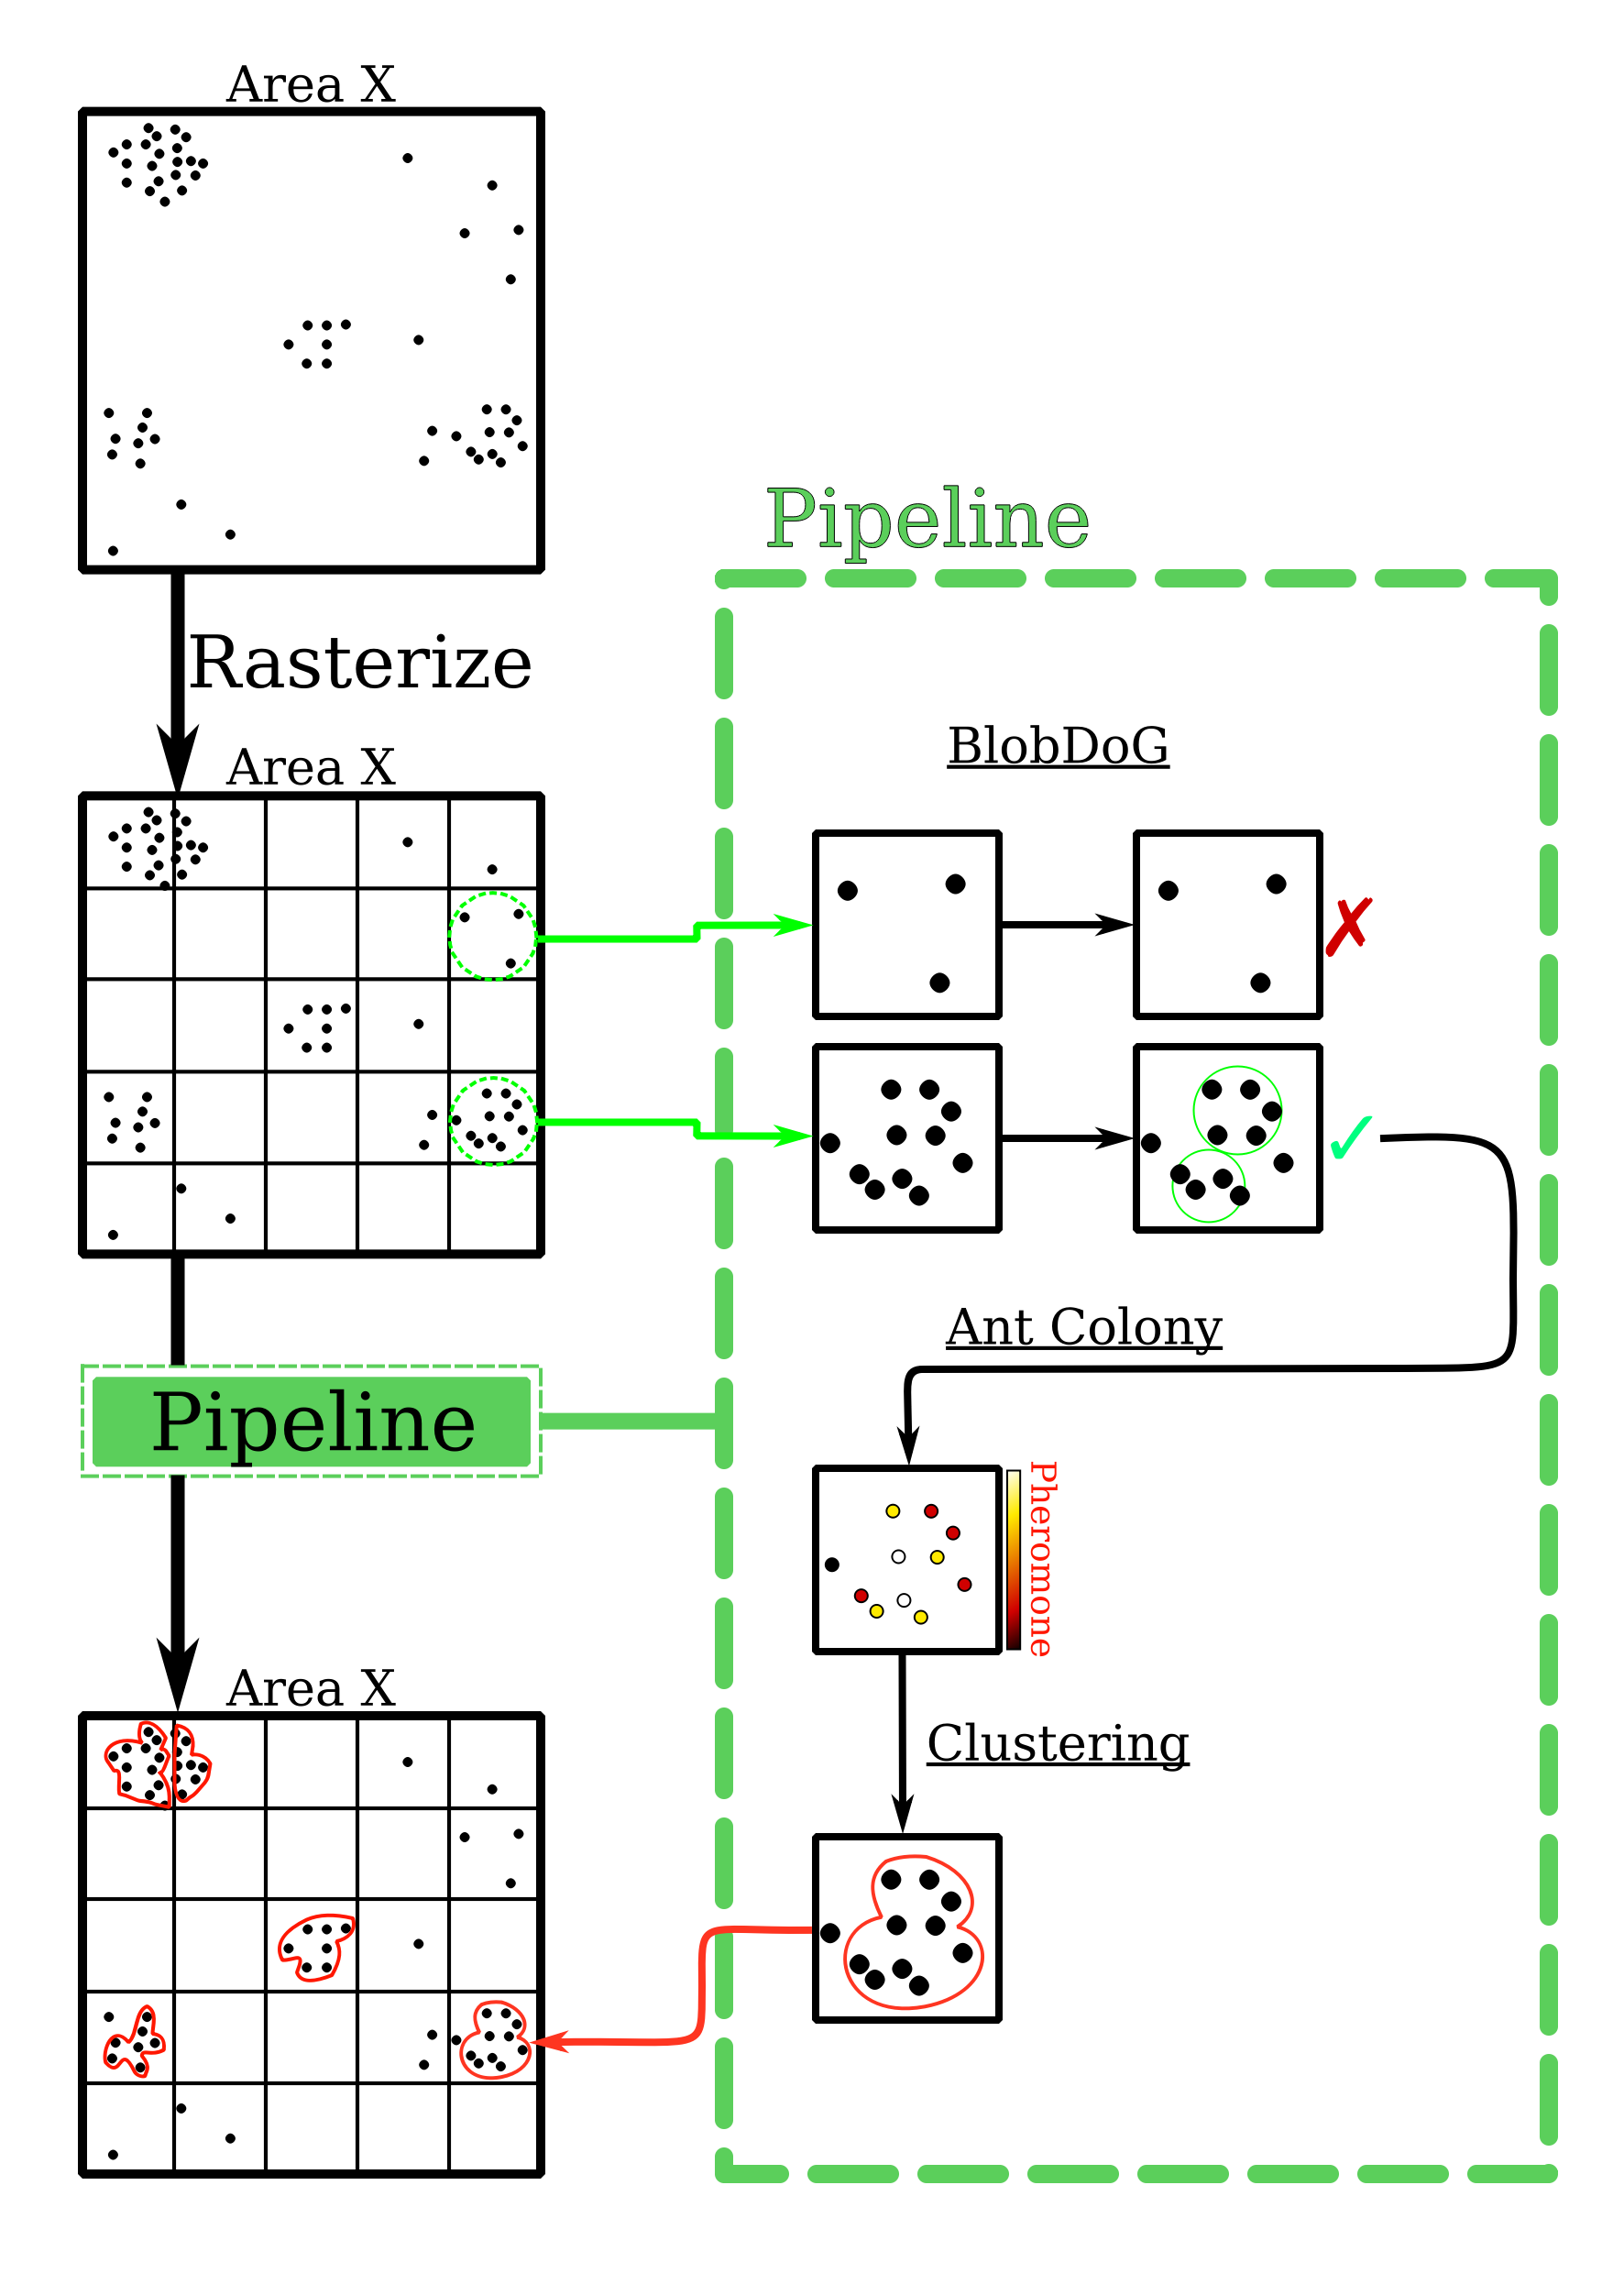
\includegraphics[height=0.75\textwidth]{figures/graphics/pipeline.png}
    \caption{\label{fig:pipeline-visualization} Overview of GC Identification}
\end{figure}
\newpage{}
\section{\label{sec:rasterization}Rasterization}

Rasterization involves splitting an area into
smaller equally sized regions. Theoretically, rasterization could occur
across any set of parameters. However, in this instance the rasterization is
applied across the equatorial coordinate system, and so the splitting is based
on the RA and Dec.

The largest known GC spans a $\text{RA}\times\text{Dec}$ of
$\SI{1.5}{\degree}\times\SI{1.5}{\degree}$~\cite{listGC} which defines the minimum
possible bound of the rasters. In, the work of Mohammadi et al., rasters of
$\SI{3.0}{\degree}\times\SI{3.0}{\degree}$ were used~\cite{Mohammadi}. However, to
account for the extraordinary case of two globular clusters of size
$\SI{1.5}{\degree}\times\SI{1.5}{\degree}$ being next to each other, rasters of size
$\SI{4.0}{\degree}\times\SI{4.0}{\degree}$ were chosen. Note, Area 2 is an outlier
due to its size and its stellar density. Thus, to explore the impact of the
\textit{denseness} of the region on the results, Area 2 is investigated with
rasterization in $\text{RA}\times\text{Dec}$ of both $\SI{2.0}{\degree}\times\SI{2.0}{\degree}$ and
$\SI{4.0}{\degree}\times\SI{4.0}{\degree}$. Figure~\ref{fig:rasterization-example}, shows an example
of rasterization applied across the Small Magellanic Cloud in Area 3.
\begin{figure}[H]
    \centering
    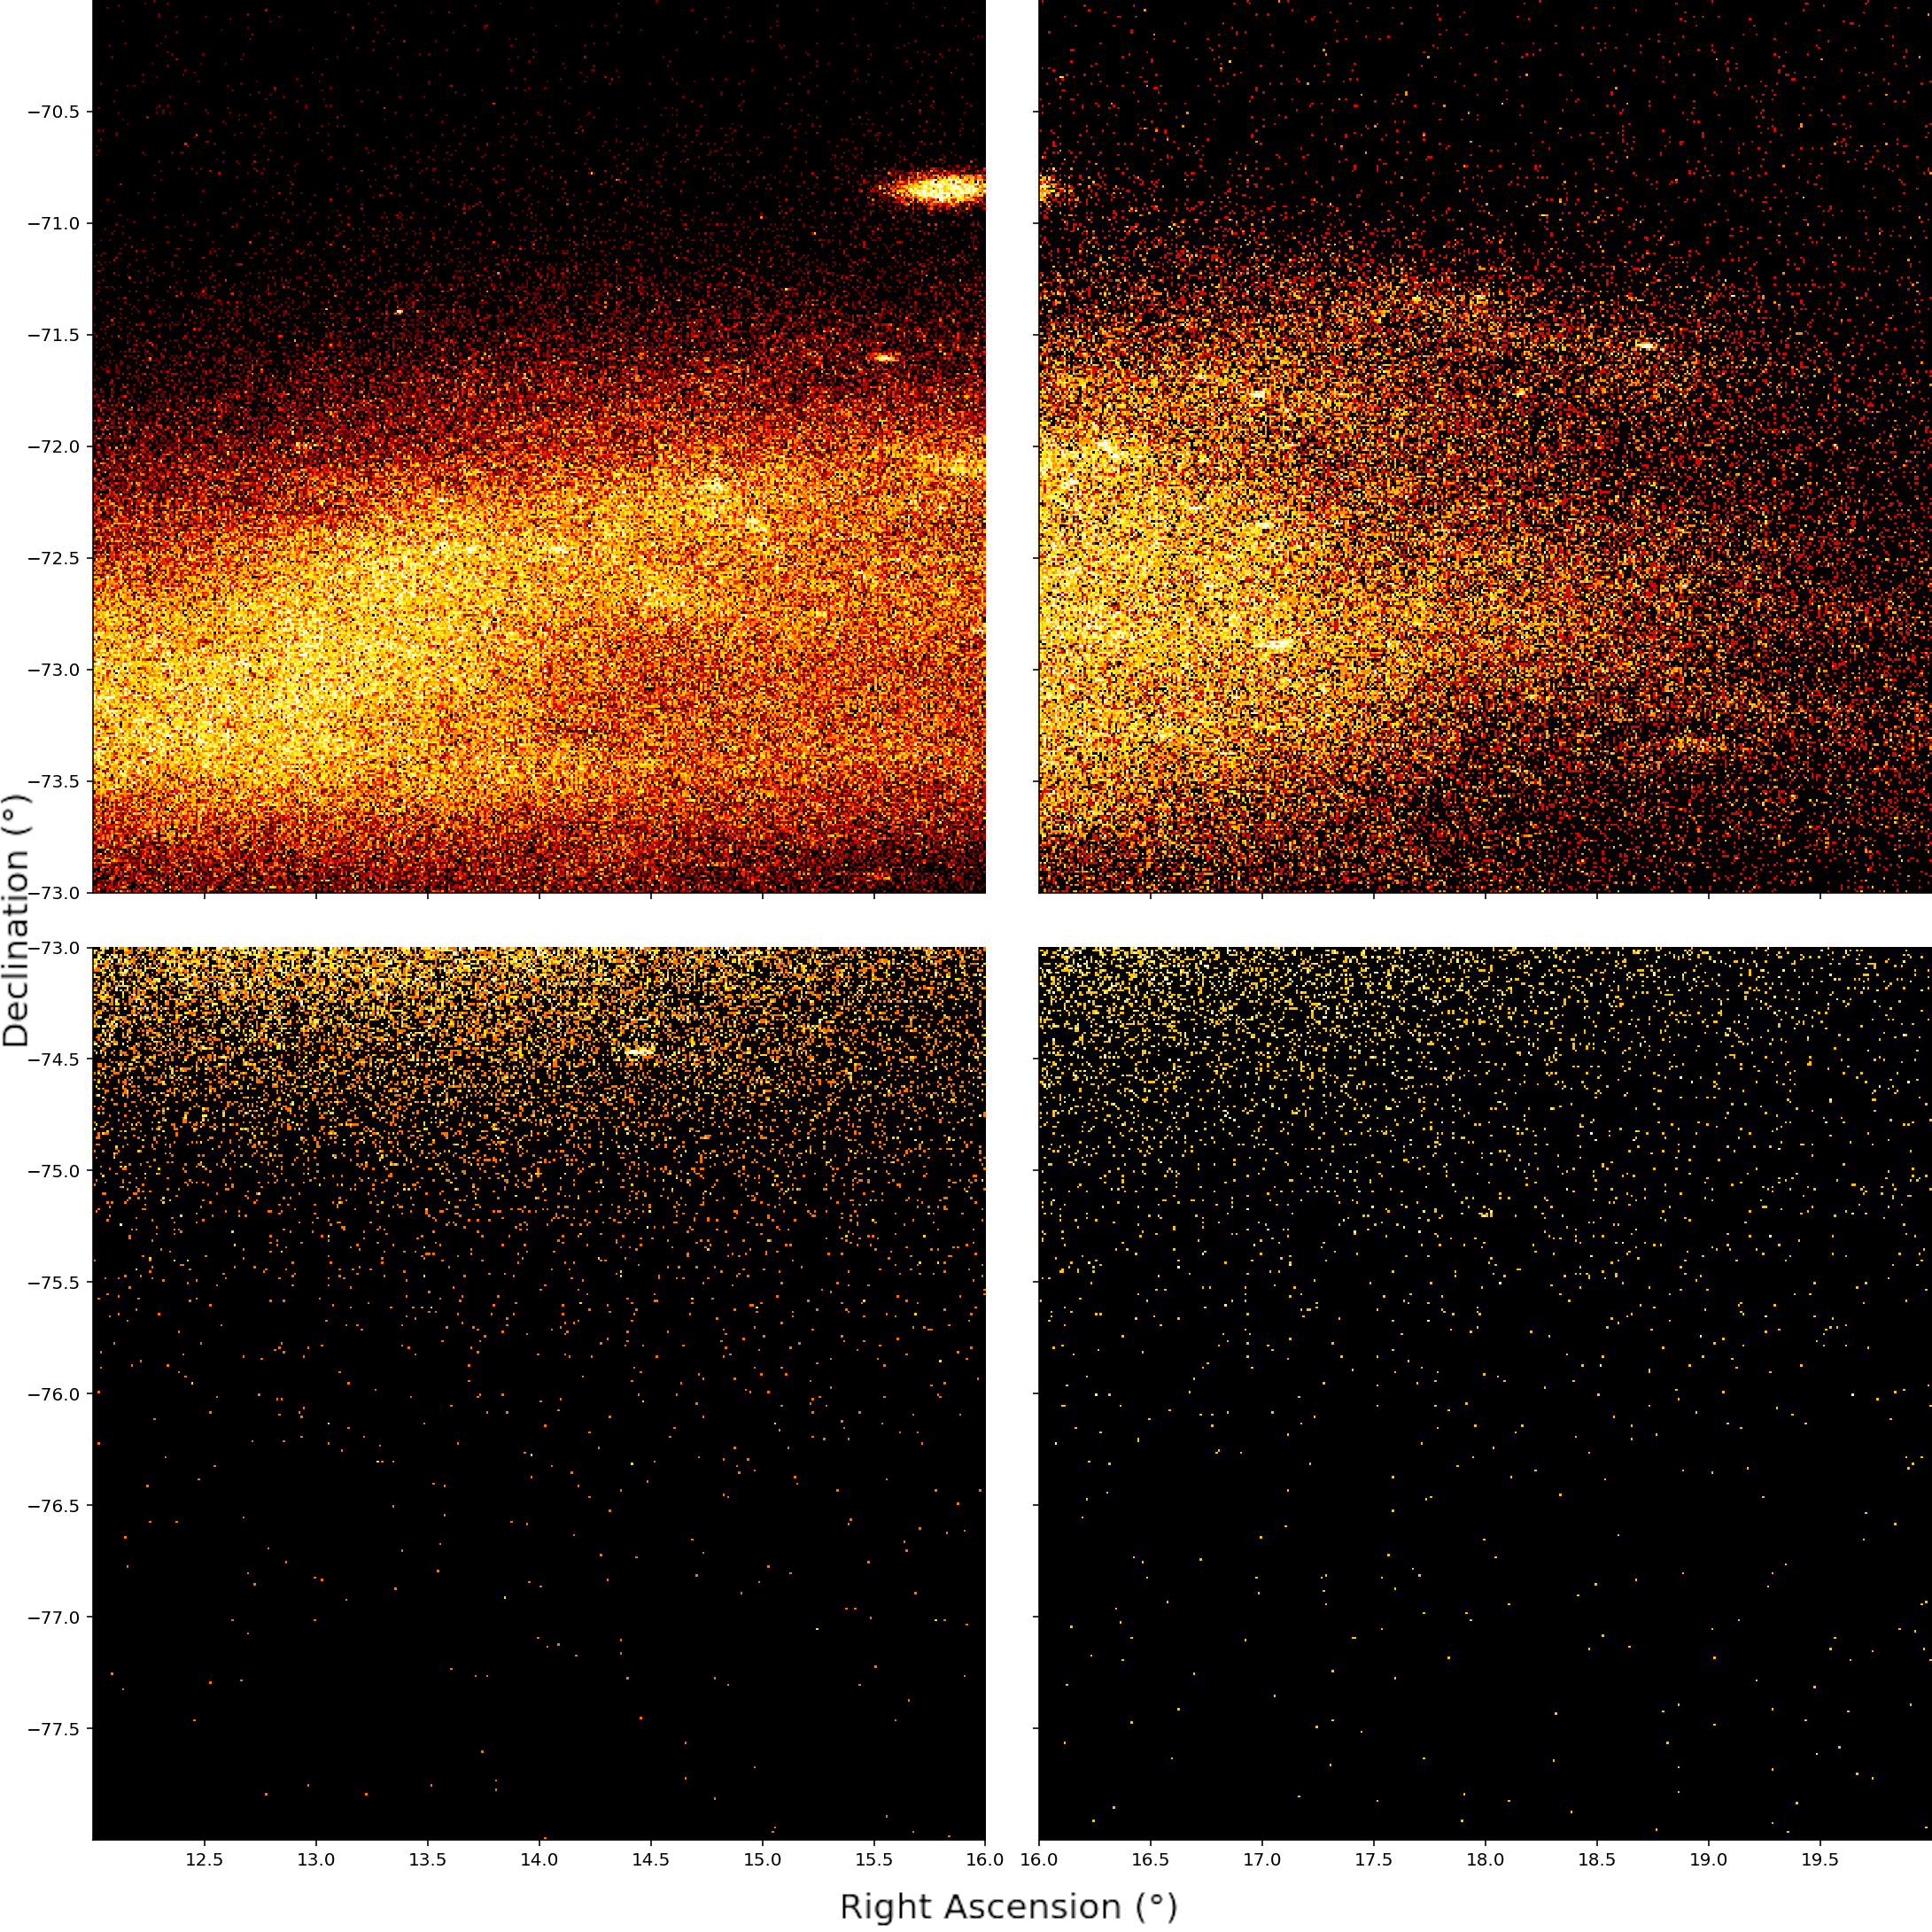
\includegraphics[width=0.85\textwidth]{rasterization/small-magellanic-cloud.png}
    \caption{\label{fig:rasterization-example} Example of Rasterization Across the Magellanic Cloud in Area 3}
\end{figure}
\vspace{-1.5em}
\noindent Rasterizing each area into smaller windows brings several benefits.
\begin{enumerate}
    \item The Ant Colony algorithm functions better on smaller regions as it is
          more easily able to explore the state space (see Section~\ref{sec:Ant} for more information).
    \item The sheer size of the data-set means that a substantial amount of
          computer memory is required to completely load one of the four areas. The
          smaller regions generated by the rasterization significantly lowers the operating memory
          requirements.
    \item Smaller regions are more likely to be empty, and get marked
          as such by the blob detection. This means that the more computationally expensive
          stages of the pipeline need to process less data.
    \item Lastly, since each raster is considered independently across the
          future stages of the pipeline, they may be operated on in parallel. This
          reduces the amount of time needed to execute the pipeline.
\end{enumerate}
However, this fixed rasterization scheme raises the issue of splitting a GC
apart at the raster boundary. This shortcoming and possible solutions are
elaborated on in Chapter~\ref{chap:evaluation}.
\newpage{}
\section{\label{sec:DoG}Raster Exclusion Using \blobdog{}}

The rasterization results in many smaller regions, upon which, the central
pipeline runs. However, the stellar distribution across these rasters
is obviously non-uniform. Figure~\ref{fig:raster-brightness} displays three
different scenarios which dominate the description of the rasters.

\begin{figure}[H]
    \centering
    \begin{subfigure}[b]{0.31\textwidth}
        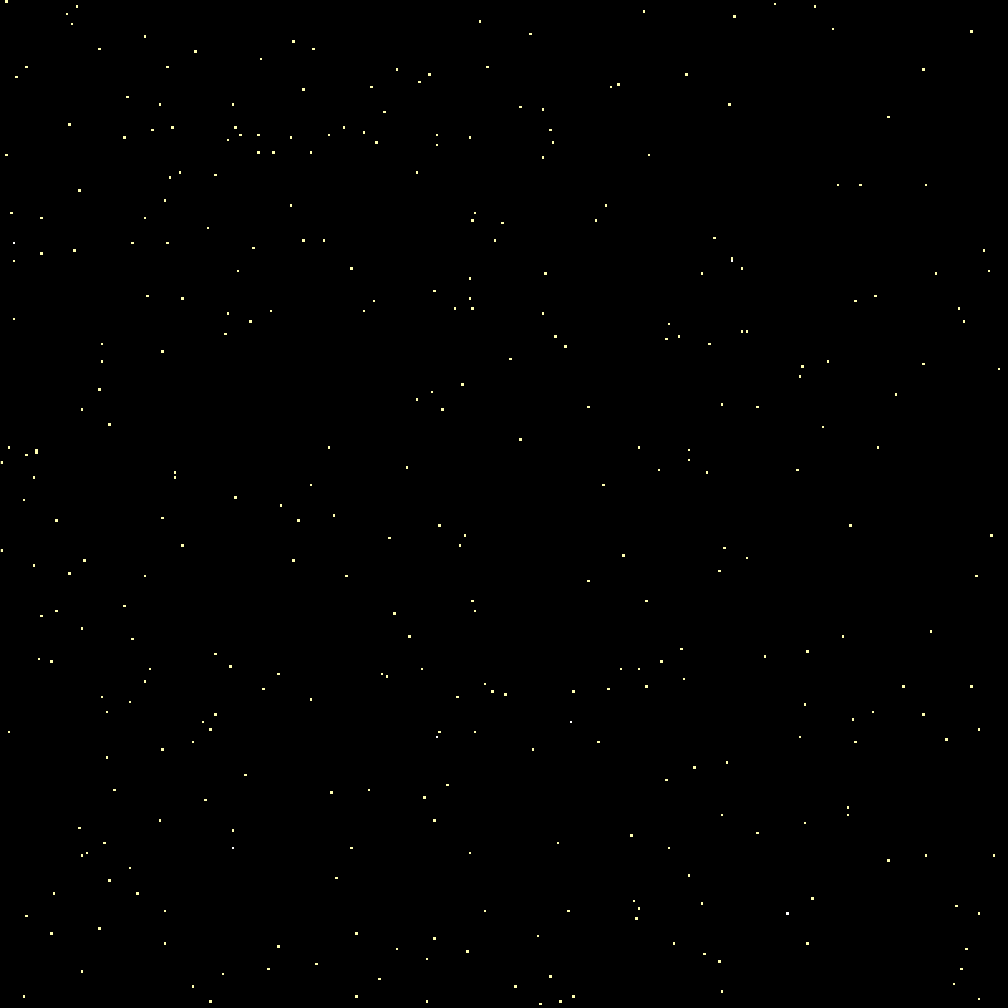
\includegraphics[width=\textwidth]{img/a1-120.0-30.0.png}
        \caption{\label{fig:dark-region}Dark Region}
    \end{subfigure}
    \hspace{0.02\textwidth}
    \begin{subfigure}[b]{0.31\textwidth}
        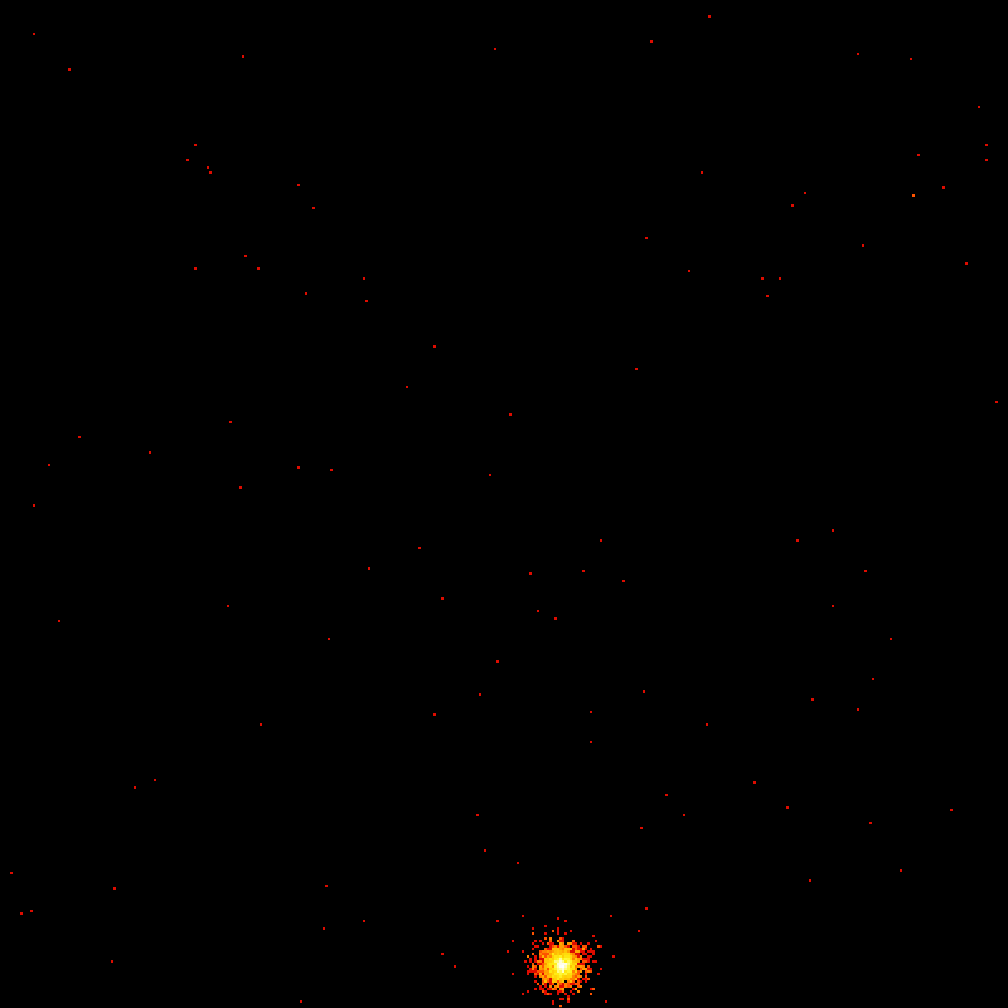
\includegraphics[width=\textwidth]{img/a1-196.0-18.0.png}
        \caption{\label{fig:dark-region-bright-spot}Dark Region with Bright Spot}
    \end{subfigure}
    \hspace{0.02\textwidth}
    \begin{subfigure}[b]{0.31\textwidth}
        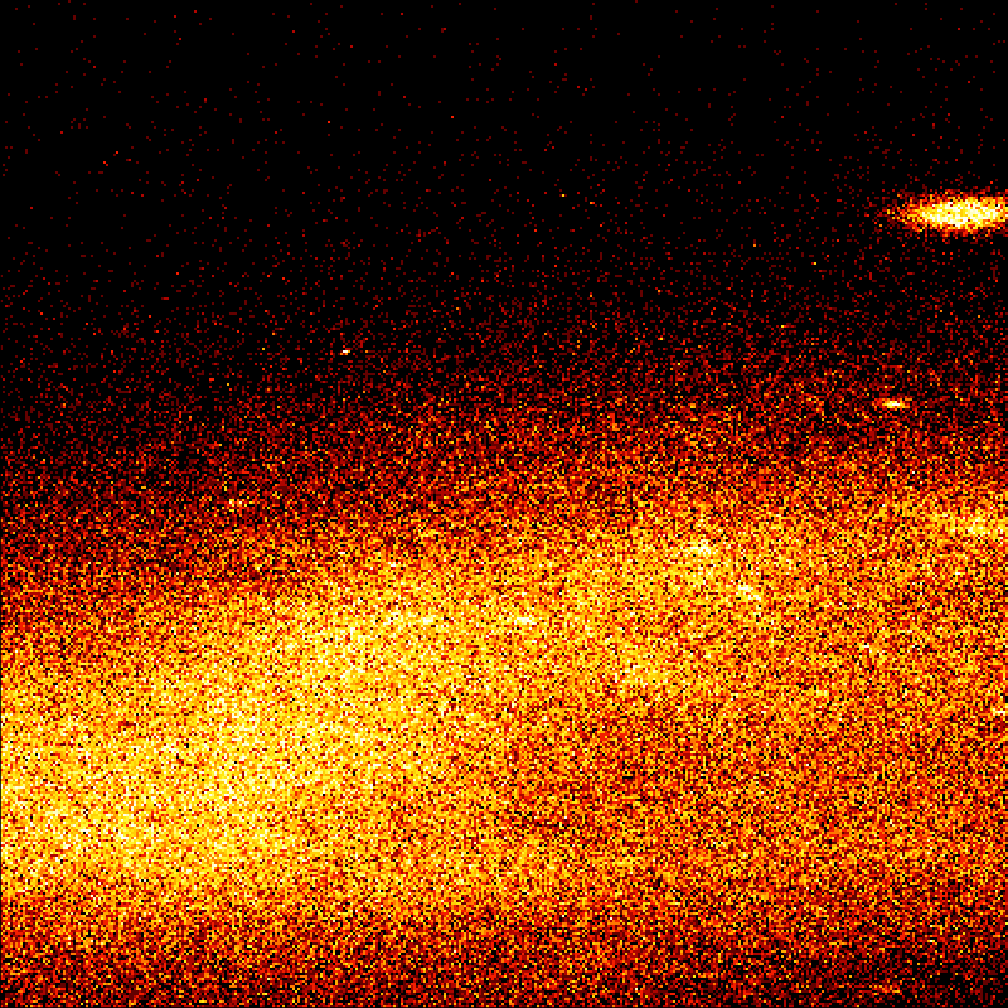
\includegraphics[width=\textwidth]{img/a3-12.0--74.0.png}
        \caption{Bright Region}
    \end{subfigure}
    \caption{\label{fig:raster-brightness} Three Types of Rasters}
\end{figure}

Given the time complexity of the Ant Colony algorithm and the
clustering algorithm, it is prudent to reduce the number of rasters to be
processed. This is done by filtering out the \textit{dark} regions similar
to the region presented in Figure~\ref{fig:dark-region}. Previous research by Mohammadi et al. made use of a blob-detection technique based on the
Difference of Gaussian~(\blobdog{}) as a post-processing
method~\cite{Mohammadi}. However, for this research, the blob detection technique is instead applied as a pre-processing step.

The \blobdog{} algorithm is provided a grayscale image and then reports information on the coordinates and size of blobs contained with that image. For a given raster, the RA, Dec, and Magnitude of stars are used to construct its grayscale representation. This results in an image where each pixel of the image has a
grayscale luminance corresponding to the magnitude. \blobdog{} is then applied on
each of these images. Rasters for which \blobdog{} reports no blobs correspond to dark regions and are filtered away.

\subsection{Components of the \blobdog{} Algorithm}
\subsubsection{\label{sec:gaussian-filters}Gaussian Filters}

\blobdog{} makes use of Gaussian filters~\cite{Lowe2004}. This technique is
fundamental to edge detection and involves the application of a Gaussian kernel
on some 2-dimensional grayscale image~$I(x, y)$ to result in a
\textit{blurred} image~\cite{gaussianKernel}. The Gaussian kernel used for this
blurring may be seen in Eq~\eqref{eq:gaussian-kernel}.
\begin{equation}
    G(x,y, \sigma) = \frac{1}{(\sqrt{2\pi}\sigma)^{2}} \exp\left(-\frac{x^{2} + y^{2}}{2\sigma^{2}}\right)
    \label{eq:gaussian-kernel}
\end{equation}
In Eq~\eqref{eq:gaussian-kernel}:
\begin{itemize}
    \item $x$ and $y$ together, represent the coordinates of a specific pixel within the image $I(x, y)$~\cite{molecularDoG},
    \item $\sigma$ represents the standard deviation of the Gaussian distribution, characterizing the width of the Gaussian kernel~\cite{molecularDoG}.
\end{itemize}
This kernel is then applied on some image
via the \textit{convolution} operation (represented by $*$), i.e.
\begin{equation*}
    I_{\text{blurred}}(x, y) = I(x, y) * G(x, y, \sigma)
\end{equation*}
Upon application, each pixel within the
image receives a weighted average of the pixels around it. The initial weights
for these surrounding pixels are determined by the Gaussian distribution
parameterized by $\sigma$. The higher the $\sigma$ value, the higher the weights allocated
to (further-away) neighbors, which ultimately results in a stronger blur.
Figure~\ref{fig:lenna-gaussian-filter} is an example of the application of this
Gaussian blurring on a well-known standard test image of Lenna Forsén~\cite{wikimedia-lenna}.

\begin{figure}[H]
    \centering
    \begin{subfigure}{0.32\textwidth}
        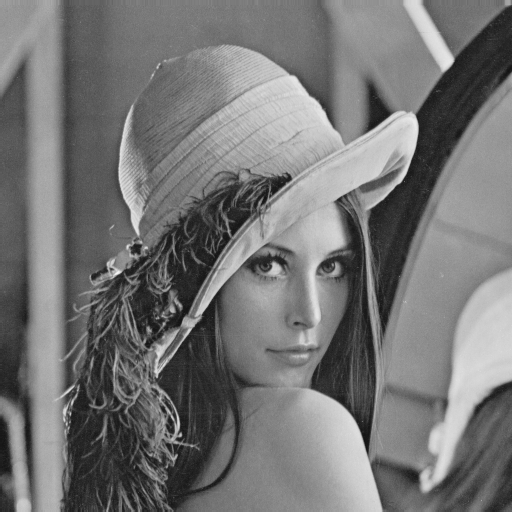
\includegraphics[width=\textwidth]{lenna/lenna-grayscale.png}
        \caption{\label{fig:lenna-original}$I(x, y)$}
    \end{subfigure}
    \begin{subfigure}{0.32\textwidth}
        
\includegraphics[width=\textwidth]{lenna/lenna-gaussian-1.png}
        \caption{\label{fig:lenna-gaussian-1} $I(x, y) * G(x, y, \sigma=2.5)$}
    \end{subfigure}
    \begin{subfigure}{0.32\textwidth}
        
\includegraphics[width=\textwidth]{lenna/lenna-gaussian-2.png}
        \caption{\label{fig:lenna-gaussian-2} $I(x, y) * G(x, y, \sigma=5.0)$}
    \end{subfigure}
    \caption{\label{fig:lenna-gaussian-filter} Gaussian Blurring applied on $I(x, y) = \text{Lenna}$}
\end{figure}
Regions within the image that have a sharp contrast have a more pronounced blur, and regions that are more uniform are affected less by the blurring. This results in a
blur that preserves boundaries and edges. It is this property that makes Gaussian filters effective in edge detection.

\subsubsection{\label{sec:difference-of-gaussian}Difference of Gaussian}

The technique used for edge detection based on Gaussian filters is the
Difference of Gaussian (DoG). As the name implies, DoG is simply the difference between the application of two different Gaussian filters on the same image, $I(x, y)$. The formula for a DoG filter may be seen in
Equation \eqref{eq:difference-of-gaussian}.
\begin{equation}
    \begin{aligned}
        DoG(x, y, \sigma) & = I(x, y) * G(x, y, k\sigma) - I(x, y) * G(x, y, \sigma)    &                                                                            & \\
                          & = I(x, y) * \left(G(x, y, k\sigma) - G(x, y, \sigma)\right) & \text{\hspace{-1em}\footnotesize Convolution distributes over subtraction} &
    \end{aligned}
    \label{eq:difference-of-gaussian}
\end{equation}

The two filters are differentiated by the presence of $k$, a constant multiplicative factor operating on the $\sigma$. As this factor increases, the strength of the blur that the corresponding Gaussian filter manifests, also increases.
The difference between these two different applications of the Gaussian filters, then causes~~\cite{Marr1980}:
\begin{itemize}
    \item the more uniform regions which maintain their similarity to be inhibited,
    \item the more distinct regions which demonstrate a stronger blur to be excited.
\end{itemize}
Fundamentally, it may be viewed as a band-pass filter that attenuates the spatial frequencies within the original image~\cite{molecularDoG}. Figure~\ref{fig:lenna-difference-of-gaussian} demonstrates the application of DoG on the image of Lenna and highlights the utility of DoG for edge detection.

\begin{figure}[H]
    \centering
    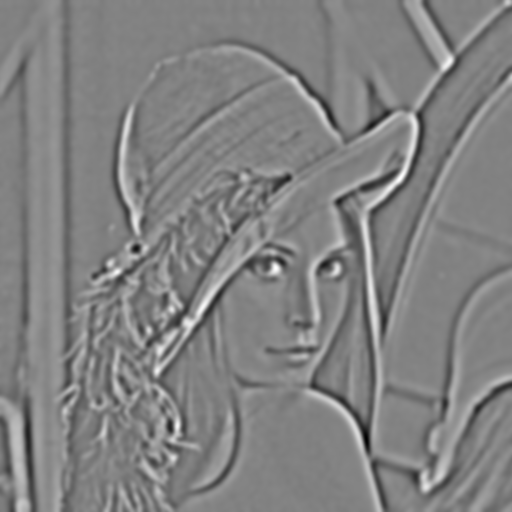
\includegraphics[width=0.32\textwidth]{lenna/lenna-difference-of-gaussian.png}
    \caption{\label{fig:lenna-difference-of-gaussian} Difference between Gaussian Blurring of Figure~\ref{fig:lenna-gaussian-1} and Figure~\ref{fig:lenna-gaussian-2}}
\end{figure}
DoG provides a mechanism to emphasize the edges of the blobs contained within a stellar raster. By identifying these boundaries at different scales the blob detection is able to report on the existence of blobs within a raster.

\subsubsection{\label{sec:blob-detection}Blob Detection}

The implementation of \blobdog{} which was used for this paper comes from the Python library \tx{SciKit}~\cite{scikit-learn}.
Their implementation is based on the work of Lowe~\cite{Lowe2004} and uses DoG to evaluate the frequency response of each pixel within an image at different scale-factors. The values for these scale-factors are proportional to the $k$ present in Eq~\eqref{eq:difference-of-gaussian}. The subsequent applications of DoG at these different scale-factors form a cube of sorts~\cite{Lowe2004}, a depiction of which, may be seen in Figure~\ref{fig:blob-dog-application}.
\begin{figure}[H]
    \centering
    \begin{subfigure}[b]{0.45\textwidth}
        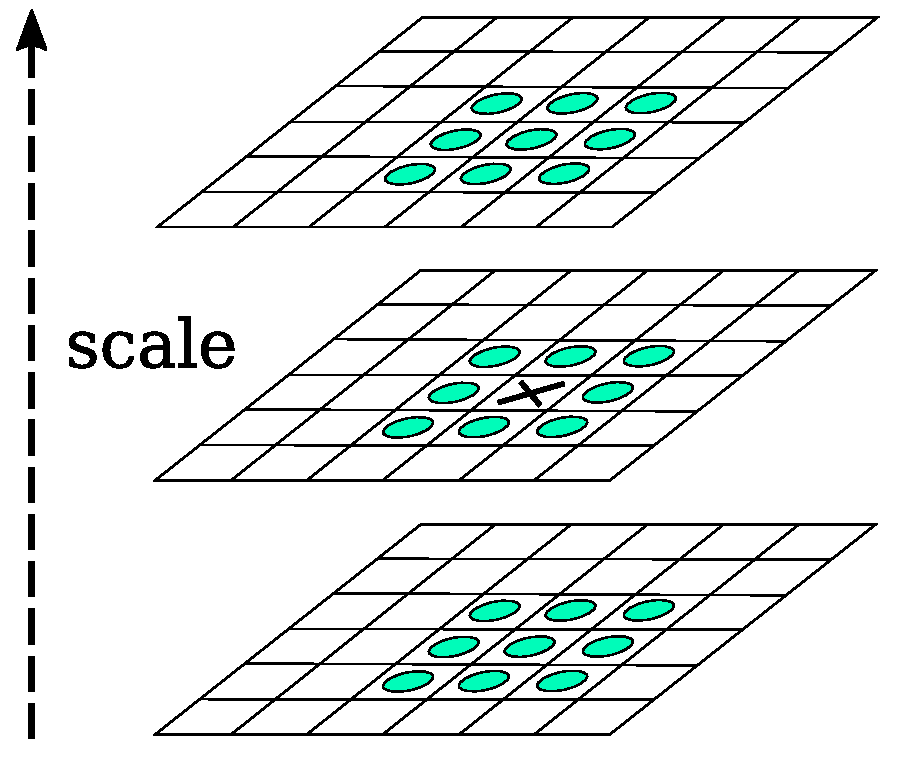
\includegraphics[height=0.70\textwidth]{graphics/blob-dog-initial.pdf}
        \caption{\label{fig:blob-dog-initial} Pixel-by-Pixel Evaluation of \blobdog{} Cube}
    \end{subfigure}
    \begin{subfigure}[b]{0.45\textwidth}
        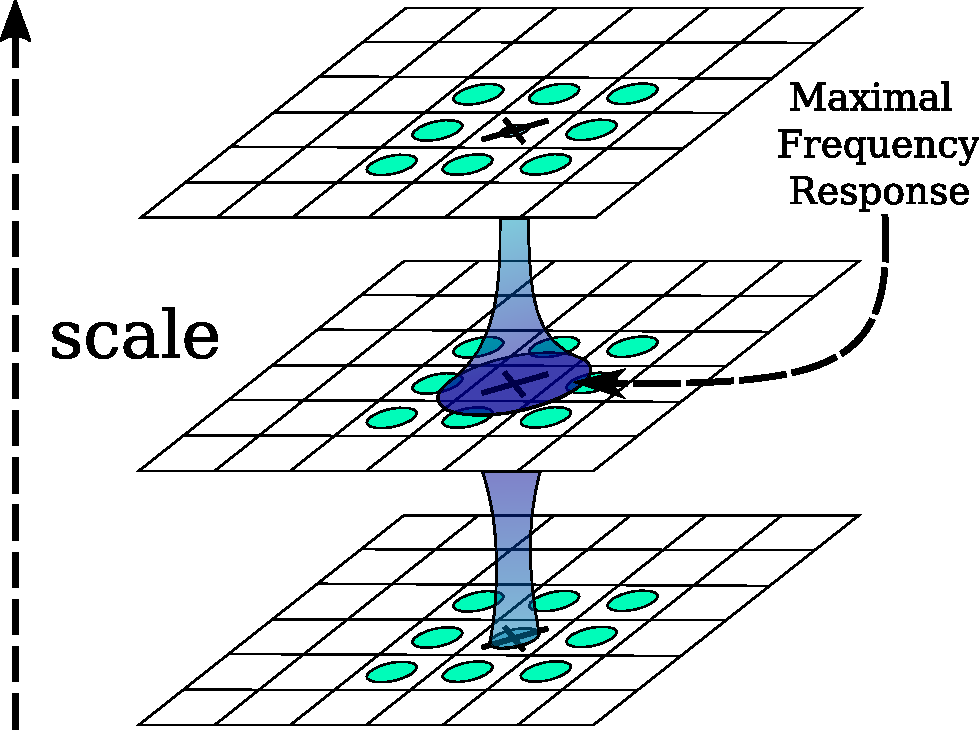
\includegraphics[height=0.70\textwidth]{graphics/blob-dog-frequency-response.pdf}
        \caption{\label{fig:blob-dog-maximal} Maximal Frequency Response}
    \end{subfigure}
    \caption{\label{fig:blob-dog-application} Application of \blobdog{}}
\end{figure}
\vspace{-1.5em}
The cross within Figure~\ref{fig:blob-dog-initial} represents the current pixel being evaluated. Its maximal frequency response is determined by comparing its response, against the 26 surrounding neighbors represented by the circles~\cite{Lowe2004}. The scale that results in the overall maxima for a pixel corresponds to the size of the largest cohesive \textit{blob} that contains that pixel. The radius of the resulting blob equates to~\cite{scikit-learn}:
\begin{equation}
    \label{eq:blob-scale}
    \text{radius} = \sqrt{2}*\text{scale}
\end{equation}
\indent{}The process in Figure~\ref{fig:blob-dog-maximal} is akin to finding the right focus for a pair of binoculars when looking at some specific point. The clarity of the image is analogous to the frequency response. As the frequency response increases, the clarity of the image increases. This continues until the maximal clarity is reached for that point at some specific focus level (the scale). Past this point the frequency response decreases and the clarity of the image begins to go down. This essentially identifies the scale at which each point becomes of interest.

Finally, the implementation uses a threshold to prune away blobs whose maximal frequency is deemed too low, as this corresponds to a blob that is too small~\cite{scikit-learn}. This threshold is represented by $B_{\text{threshold}}$ and its value is elaborated on in Section~\ref{sec:constants}.

\subsection{Interpreting the Results of \blobdog{}}
\blobdog{} provides information on the position and scale of any blob that is sufficiently large (based on $B_{\text{threshold}}$). If no blobs are detected then that raster may be filtered away. Using Eq\textrm{~}\eqref{eq:blob-scale} the radii of any blobs are determined and this is used to plot the results. Figure~\ref{fig:dog-raster} shows the results of \blobdog{} when applied on the exemplar rasters that were shown in Figure~\ref{fig:raster-brightness}.
\begin{figure}[H]
    \centering
    \begin{subfigure}[b]{0.31\textwidth}
        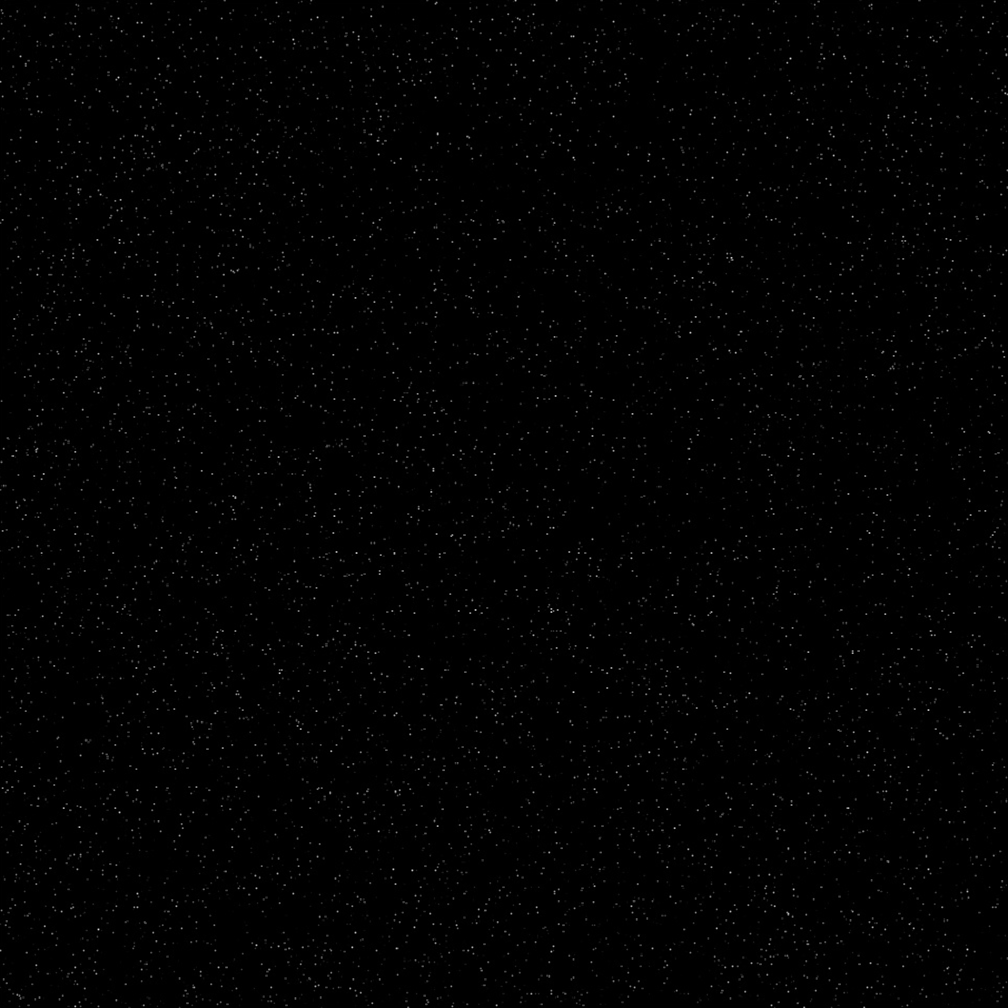
\includegraphics[width=\textwidth]{img/dog-a1-120.0-30.0.png}
        \caption{\label{fig:dog-dark-region}Dark Region}
    \end{subfigure}
    \hspace{0.02\textwidth}
    \begin{subfigure}[b]{0.31\textwidth}
        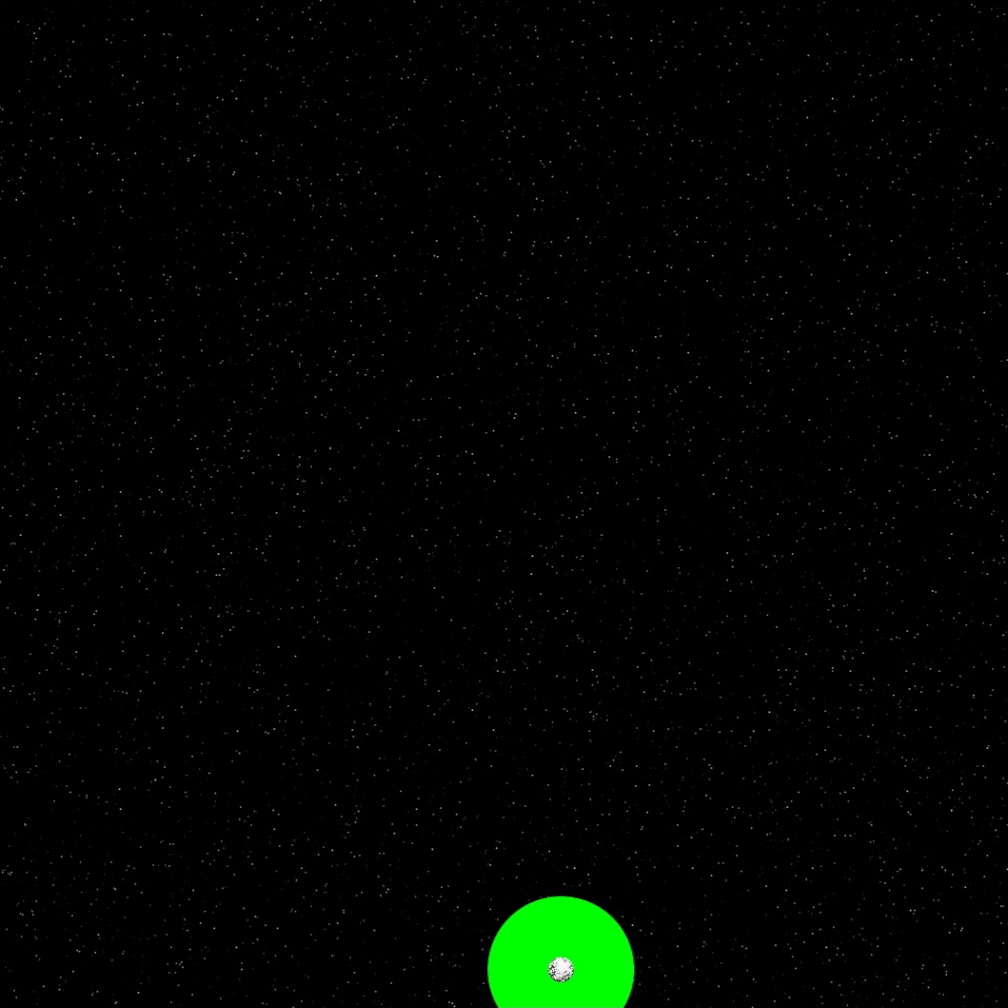
\includegraphics[width=\textwidth]{img/dog-a1-196.0-18.0.png}
        \caption{\label{fig:dog-one-blob}Dark Region with Bright Spot}
    \end{subfigure}
    \hspace{0.02\textwidth}
    \begin{subfigure}[b]{0.31\textwidth}
        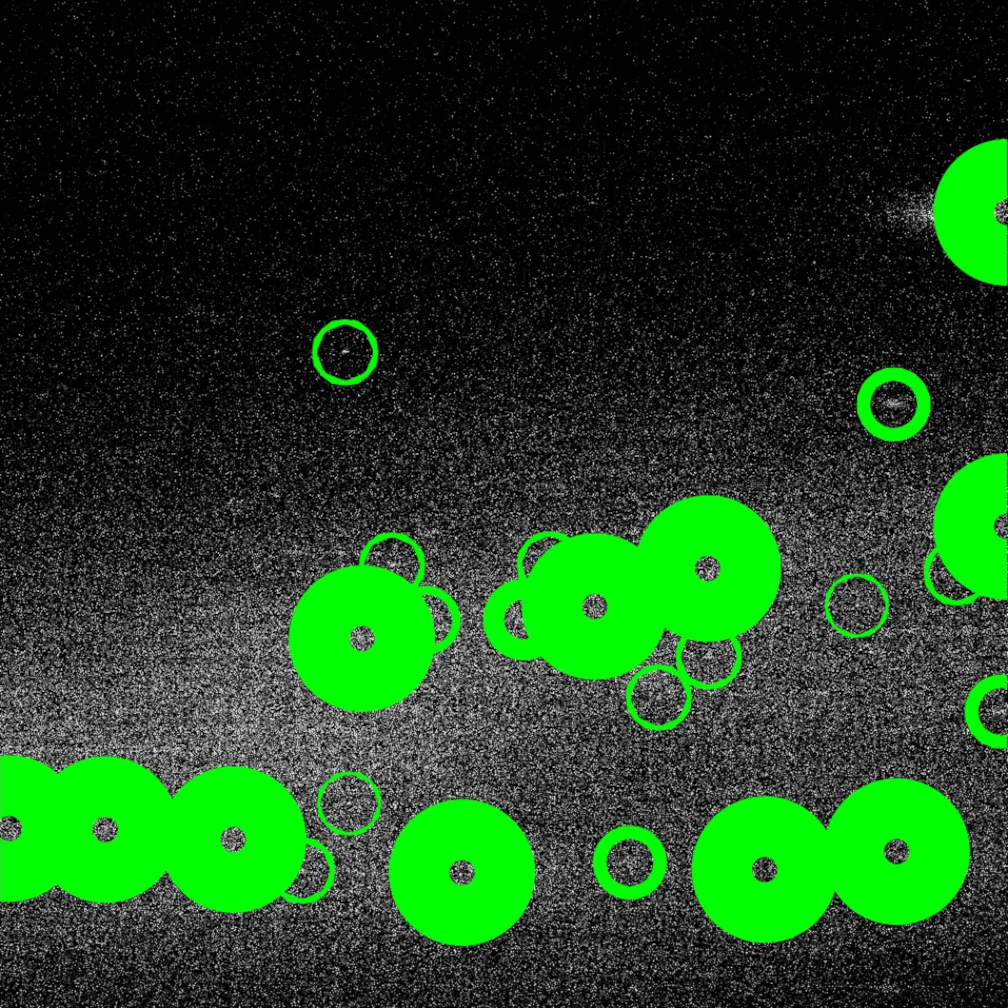
\includegraphics[width=\textwidth]{img/dog-a3-12.0--74.0.png}
        \caption{\label{fig:dog-bright-region}Bright Region}
    \end{subfigure}
    \caption{\label{fig:dog-raster} DoG Applied to the Three Types of Rasters}
\end{figure}
\vspace{-1.5em}
Since Figure~\ref{fig:dog-dark-region} contains no blobs, its corresponding raster will be filtered away. Figure~\ref{fig:dog-one-blob} and Figure~\ref{fig:dog-bright-region} contain one or more blobs and their rasters should be processed by the future stages of the pipeline.
\newpage{}
\section{\label{sec:Ant}Density Mapping Via the Ant Colony}

With the initial filtration handled by \blobdog{}, what remains is the task of identifying potential GCs in the rasters that have persisted. It is difficult to precisely encode the properties of GCs such that an exhaustive search algorithm could identify them in a timely fashion. Instead we aim to produce density mappings and cluster the densest regions in a fashion similar to what was done in the previous work by Mohammadi et al.~\cite{Mohammadi}.

Since GCs are an agglomerate structure, when identifying them, it is necessary to consider the attributes of individual stars, as well as, the relationship between stars. To this end, it is possible to re-frame the scenario and represent the stars on a graph, with the stars representing the nodes and the relationships between the stars represented as edges. Encoding these edges with weights based on the similarities between the pairs of stars provides a foundation for the use of the \textit{Ant Colony random-walk} algorithm.

This algorithm is based on the swarm behavior that manifests in biological ant colonies~\cite{AntColony}. A swarm of ants explores a region by (randomly) discovering the shortest routes to a desirable resource and then leaving \textit{pheromone} trails for other ants to follow. As other ants follow this path and also discover this same resource, the pheromone trail becomes stronger, continuing to attract more and more ants until the resource is consumed. These pheromone values naturally decay over time and allow the ant colony to dynamically optimize their routes based on their environmental context~\cite{AntColony}.

After the ants have been provided a sufficient amount of time to explore, these pheromone values will result in a random path that approximately describes the network substructure of their environment~\cite{Xia2019}. The strength of these pheromone trails provide us the density mapping which will be used to cluster candidate GCs (as described in Section~\ref{sec:Clustering}).

\subsection{Components of the Ant Colony Algorithm}

The core algorithm for the Ant Colony may be seen in Alg.\,\ref{alg:ant-colony}. Note that the values that were selected for the constants $N_{\text{gens}}$, $N_{\text{ants}}$, and $N_{\text{steps}}$ may be found in Section~\ref{sec:constants}.
\vspace{-0.4em}
\begin{algorithm}[H]
    \caption{\label{alg:ant-colony}Ant Colony~\cite{AntColonyMohammadi}}
    \footnotesize{}
    \begin{algorithmic}
        \Ensure{The pheromone vector: $\mathbf{f} = \left[f_{1}, f_{2}, \dots, f_{N_{\text{stars}}}\right]$}

        \begin{minipage}{\columnwidth{}}
            \hspace{-5em}
            \vhrulefill{0.3pt}
        \end{minipage}
        \State{$\mathbf{f}^{0} = \left[0, 0, \dots, 0\right]$}
        \Comment{Length of $N_{\text{stars}}$.}
        \For{$t = 1, \dots, N_{\text{gens}}$}
        \State{$\mathbf{N^{t-1}_{\text{visitations}}} = \left[0, 0, \dots, 0\right]$}
        \Comment{Length of $N_{\text{stars}}$.}
        \For{$\text{ant} = 1, \dots, N_{\text{ants}}$}
        \State{$\text{star} \gets$ Random initial position for the $\text{ant}$, based on a uniform random distribution.}
        \State{$\mathbf{N^{t-1}_{\text{visitations}}}\left[\text{star}\right] \pluseq{} 1$}
        \For{$\text{step} = 1, \dots, N_{\text{steps}}$}
        \State{$\text{star} \gets$ Random next position for the \text{ant}, weighted by the transition probability: Eq.~\eqref{eq:transitionProbability}}
        \Comment{This uses \\\hphantom{mmmmmmmmmmmmmmmmmmmmmmmmmmmmmmmmmmmm}$\text{star}$ (the current position) and $\mathbf{f}^{t-1}$.}
        \State{$\mathbf{N^{t-1}_{\text{visitations}}}\left[\text{star}\right] \pluseq{} 1$}\phantom{$N_{V_{V_{V}}}$}
        \EndFor{}
        \EndFor{}
        \State{Update $\mathbf{f}^{t-1}$ to $\mathbf{f}^{t}$ using the pheromone update function: Eq.~\eqref{eq:updatePheromone}}
        \Comment{This uses $t$, $\mathbf{f}^{t-1}$, $\mathbf{N^{t-1}_{\text{visitations}}}$, $N_{\text{ants}}$, and\\\hphantom{mmmmmmmmmmmmmmmmmmmmmmmmmmmmmmmmmmmm}$N_{\text{steps}}$.}
        \EndFor{}
        \State{\Return{$\mathbf{f}^{N_{\text{gens}}}$}}
    \end{algorithmic}
\end{algorithm}
\vspace{-1.2em}
Before any ants can take their first steps, the feature vector $\mathbf{f}$ containing a pheromone value for each star is initialized. The main logic of the algorithm is comprised of a triple nested loop. The outermost loop represents an iteration over a number of generations ($N_{\text{gens}}$). Each subsequent generation is able to make use of the information from the previous generation thereby thoroughly exploring the state space and allowing for more accurate, average pheromone values. This outer loop executes three steps:
\begin{enumerate}
    \item The initialization of $\mathbf{N_\text{visitations}}$ keeps track of the number of visits to each star.
    \item The inner loop where a number of ants corresponding to $N_\text{ants}$ are set loose randomly within the stellar raster.
    \item The transitioning of the pheromone values between each experiment using the pheromone update function described by Eq.~\eqref{eq:updatePheromone}.
\end{enumerate}
The inner loop iterates across each ant and executes the random-walk for that ant. First, the ant is spawned at a random starting position. The visitation for that starting position is updated and then the ant proceeds to walk around for a number of steps (corresponding to a total of $N_{\text{steps}}$). This is represented by the innermost loop, where the ant determines its next step in a random fashion biased by the distribution of pheromones in its neighborhood. This allows it to determine its best path based on the knowledge left behind by previous ants. This step is governed by Eq.~\eqref{eq:transitionProbability}.

Finally, after all the ants have performed their random-walks, the pheromone values for that experiment may be updated. The updating of the pheromone values marks the end of one experiment, after which, the next experiment may begin. From this description, it is evident that the core of the Ant Colony algorithm is fairly simple. However, its strength hinges on the transition probability driving the core decision making process of the ants.

To compute this transition probability it is necessary to compute additional information on the relationship between stars. However, it is not feasible to compute the relationship between all pairs of stars due to the sheer number of stars. Additionally, it is not even useful to compute this data for stars that are too far apart. Thus, from a given star, $x_{i}$ an ant will only consider a limited amount of neighboring stars ($N_{\text{neighbors}}$). These neighboring stars correspond to the stars that are closest by Euclidean distance. This distance is based on the $\text{RA}$, $\text{Dec}$, and $\text{Distance}$ and for two stars $x_{i}$ and $x_{j}$ is computed as follows:
\begin{align}
    \resizebox{!}{0.8\height{}}{$%
            \begin{aligned}
                \resizebox{!}{1.2\height{}}{$\text{Euclidean Distance Between } x_{i} \text{ and } x_{j} =$}
                \biggl\{
                \Bigl(\text{RA}_{x_{i}} & - \text{RA}_{x_{j}}\Bigr)^{2}\ +                     \\
                \Bigl(                  & \text{Dec}_{x_{i}} - \text{Dec}_{x_{j}}\Bigr)^{2}\ + \\
                                        & \phantom{\text{Dec}_{x_{i}}}
                \Bigl(\text{Distance}_{x_{i}} - \text{Distance}_{x_{j}}\Bigr)^{2}
                \biggr\}^{\frac{1}{2}}
            \end{aligned}
        $%
    }
\end{align}
For the star $x_{i}$, the list of its nearest neighbors is represented as $\mathcal{N}_{x_{i}}$ and this list is assumed to be sorted in ascending order by Euclidean distance from $x_{i}$.
\vspace{-1em}
\subsection{Transition Probability}
\vspace{-0.3em}
The first step in computing the transition probability is to compute the \textit{weights} between each star and its nearest neighbors. This weight should be proportional to how rewarding it would be for an ant to make a transition from its current star to some neighboring star. For two stars, $x_{i}$ and $x_{j}$, their weight is represented by $w(x_{i}, x_{j})$. Since the main aim is to identify stars with certain similar features that may make them part of the same GC, the weight must constitute the similarity between a pair of stars. Stars within GCs are relatively near to each other and manifest similar motion characteristics. Thus, the parameters used to compute the weights are:
\vspace{-0.3em}
\begin{itemize}
    \item the $\text{RA}$, $\text{Dec}$, and $\text{Distance}$ as these parameters encode the position,
    \item the $\text{PM}_{\text{RA}}$ and $\text{PM}_{\text{Dec}}$ as these parameters encode the motion.
\end{itemize}
\vspace{-1em}
\subsubsection{\label{weight-initialization}Computing the Weights}
\vspace{-0.5em}
The algorithm used to compute the weights is as follows:
\vspace{-0.4em}
\begin{algorithm}[H]
    \caption{Computing Weights Between All Stars and Their Neighbors~\cite{scikit-learn}}
    \footnotesize{}
    \begin{algorithmic}
        \Require{The \textit{stars} where for each star, $x_{i}$, the following are accessible:
            \begin{itemize}
                \item The relevant parameters of $x_{i}$: $\text{RA}_{x_{i}}$, $\text{Dec}_{x_{i}}$, $\text{Distance}_{x_{i}}$, ${\text{PM}_{\text{RA}}}_{x_{i}}$, and ${\text{PM}_{\text{Dec}}}_{x_{i}}$
                \item The ($N_{\text{neighbors}}$) nearest neighbors of $x_{i}$: $\mathcal{N}_{x_{i}}$
            \end{itemize}
        }
        \Ensure{A lookup table for the \textit{weights}, $w$, where the weight from $x_{i}$ to $x_{j}$ may be looked-up via $w(x_{i}, x_{j})$.}
        \begin{minipage}{\columnwidth{}}
            \hspace{-5em}
            \vhrulefill{0.3pt}
        \end{minipage}
        \State{$w =$
            \begin{blockarray}{ccccc}
                & {\tiny$\mathcal{N}_{x_{i}}[1]$} & {\tiny$\mathcal{N}_{x_{i}}[2]$} & {$\dots$} & {\tiny$\mathcal{N}_{x_{i}}[N_{\text{neighbors}}]$}\\
                \begin{block}{c[cccc]}
                    {\tiny$x_{1}$} & $0$ & $0$ & $\dots$ & $0$\topstrut{} \\
                    {\tiny$x_{2}$} & $0$ & $0$ & $\dots$ & $0$ \\
                    {$\vdots$} & $\vdots$ & $\vdots$ & $\ddots$ & $\vdots$ \\
                    {\tiny$x_{N_{\text{stars}}}$} & $0$ & $0$ & $\dots$ & $0$\botstrut{}\\
                \end{block}
            \end{blockarray}
        }
        \Comment{Initialize the lookup table for the weights to $0$.}
        \For{$x_{i} \in \text{stars}$}
        \State{$D =$
            \resizebox{!}{33pt}{
                \begin{blockarray}{cccccc}
                    & {\tiny $\text{RA}$} & {\tiny $\text{Dec}$} & {\tiny $\text{Distance}$} & {\tiny $\text{PM}_{\text{RA}}$} & {\tiny $\text{PM}_{\text{Dec}}$} \\
                    \begin{block}{c(ccccc)}
                        {\tiny$\mathcal{N}_{x_{i}}[1]$} & $\text{RA}_{\mathcal{N}_{x_{i}[1]}}$      & $\text{Dec}_{\mathcal{N}_{x_{i}[1]}}$      & $\text{Distance}_{\mathcal{N}_{x_{i}[1]}}$      & ${\text{PM}_{\text{RA}}}_{\mathcal{N}_{x_{i}[1]}}$      & ${\text{PM}_{\text{Dec}}}_{\mathcal{N}_{x_{i}[1]}}$\topstrut{}      \\
                        {\tiny$\mathcal{N}_{x_{i}}[2]$} & $\text{RA}_{\mathcal{N}_{x_{i}[2]}}$      & $\text{Dec}_{\mathcal{N}_{x_{i}[2]}}$      & $\text{Distance}_{\mathcal{N}_{x_{i}[2]}}$      & ${\text{PM}_{\text{RA}}}_{\mathcal{N}_{x_{i}[2]}}$      & ${\text{PM}_{\text{Dec}}}_{\mathcal{N}_{x_{i}[2]}}$      \\
                        {$\vdots$} & $\vdots$ & $\vdots$ & $\vdots$ & $\vdots$ & $\vdots$ \\
                        {\tiny$\mathcal{N}_{x_{i}}[N_{\text{neighbors}}]$} & $\text{RA}_{\mathcal{N}_{x_{i}[N_{\text{neighbors}}]}}$      & $\text{Dec}_{\mathcal{N}_{x_{i}[N_{\text{neighbors}}]}}$      & $\text{Distance}_{\mathcal{N}_{x_{i}[N_{\text{neighbors}}]}}$      & ${\text{PM}_{\text{RA}}}_{\mathcal{N}_{x_{i}[N_{\text{neighbors}}]}}$      & ${\text{PM}_{\text{Dec}}}_{\mathcal{N}_{x_{i}[N_{\text{neighbors}}]}}$\botstrut{}     \\
                    \end{block}
                \end{blockarray}
            }
        }
        \Comment{Assign the parameters from each neighbor to the feature matrix, $D$.}
        \\
        \State{$\overline{D} = D - \mu(D)$}
        \Comment{\hspace{0.17em}Center the data by subtracting column-wise means so the mean of each column is $0$.}
        \State{$U, \Sigma, V^{\intercal{}} = \svd(\overline{D})$}
        \Comment{Get the singular values and singular vectors from the Singular Value Decomposition.}
        \State{$\widehat{D} = \dfrac{\overline{D}}{\norm{\overline{D}}}$}
        \Comment{Compute the correlation coefficient for each star.}
        \State{$\text{weights}_{\mathcal{N}_{x_{i}}} = \abs{\widehat{D} * V} * \Sigma$}
        \Comment{$\text{weights}_{\mathcal{N}_{x_{i}}}$ is of length $N_{\text{neighbors}}$ and has one element for each neighbor of $x_{i}$.}
        \State{Insert $\text{weights}_{N_{x_{i}}}$ into row for $x_{i}$ in $w$}
        \EndFor{}
        \vspace{0.5em}
        \State{\Return{$w$}}
    \end{algorithmic}
\end{algorithm}


The aim in the weight initialization is to compute a single metric capable of uniformly representing the differences between the 5 different parameters across a pair of stars. This problem requires a form of dimensionality reduction which is done using Singular Value Decomposition (SVD)~\cite{PCA}. SVD may be used to generate an orthogonal projection to the original dimensions which minimizes the mean-squared distance of the observed points from the new basis axes. In effect this produces a linear combination of the original parameters which maintains the maximal variance of the constituent dimensions~\cite{julia-stats}.

\subsubsection{Computing the Transition Probability}
With the weights in place the ants have an initial basis for forming their decisions. However, the ants should also take into account the pheromone trails left by previous ants. By combining the underlying weights with the previous pheromone values the ants may determine a probability for transitioning to the neighboring stars~\cite{AntColonyMohammadi}.
\begin{align}
    \hat{f}^{t}(x_{j})   & = \frac{f^{t}(x_{j})}{\mathlarger{\sum\limits_{x_{k} \in \mathcal{N}_{x_{i}}}}\hspace{-0.60em}f^{t}(x_{k})}                                                                                                                                                                & \reason{Normalize the pheromone value of $x_{j}$~(a neighbor of $x_{i}$) based on the neighborhood of $x_{i}$.} \label{eq:pheromoneNormalization} \\
    \hphantom{
    P^{t}(x_{i}, x_{j})} & \hphantom{= \frac{{\Bigl(w(x_{i}, x_{j})\Bigr)}^{\gamma} {\Bigl(\hat{f}^{(t-1)}(x_{j})\Bigr)}^{1-\gamma}}{\mathlarger{\sum\limits_{x_{k} \in \mathcal{N}_{x_{i}}}}\hspace{-0.75em}{\Bigl(w(x_{i}, x_{k})\Bigr)}^{\gamma} {\Bigl(\hat{f}^{(t-1)}(x_{k})\Bigr)}^{1-\gamma}}} & \nonumber{}
\end{align}
\\
\vspace{-4.5em}

\noindent{}$\hat{f}^{t}(x_{j})$ is the normalized pheromone value of $x_{j}$ at generation $t$. It is normalized by evaluating $f^{t}(x_{j})$ (the pheromone value of $x_{j}$ at generation $t$) and then dividing it by the sum of the pheromone values of the all the stars in the neighborhood. The transition probability between $x_{i}$ and $x_{j}$ is then simply computed by mixing the weight between $x_{i}$ and $x_{j}$ and the normalized pheromone value of $x_{j}$ in the previous generation.
\begin{align}
    P^{t}(x_{i}, x_{j})           & = \frac{{\Bigl(w(x_{i}, x_{j})\Bigr)}^{\gamma} {\Bigl(\hat{f}^{(t-1)}(x_{j})\Bigr)}^{1-\gamma}}{\mathlarger{\sum\limits_{x_{k} \in \mathcal{N}_{x_{i}}}}\hspace{-0.75em}{\Bigl(w(x_{i}, x_{k})\Bigr)}^{\gamma} {\Bigl(\hat{f}^{(t-1)}(x_{k})\Bigr)}^{1-\gamma}} & \reason{Compute the transition probability of going from $x_{i}$ to $x_{j}$.} \label{eq:transitionProbability} \\
    \hphantom{\hat{f}^{t}(x_{j})} & \hphantom{= \frac{f^{t}(x_{j})}{\mathlarger{\sum\limits_{x_{k} \in \mathcal{N}_{x_{i}}}}\hspace{-0.60em}f^{t}(x_{k})}}                                                                                                                                          & \nonumber{}
\end{align}
\\
\vspace{-4.5em}

\noindent{}%
$P^{t}(x_{i}, x_{j})$ is the transition probability from $x_{i}$ to $x_{j}$ computed for generation $t$. In the equation, $\gamma$ is a control parameter that simply determines the relative impact of the weights versus the pheromone values (see Section~\ref{sec:constants} for information on the value selected for $\gamma$). The range for $\gamma$ is $0~\leq~\gamma~\leq~1$.
\begin{itemize}
    \item $\gamma = 0$ describes a scenario where the pheromone values are all that are involved in determining the transition probability.
    \item $\gamma = 1$ describes a scenario where the weights are the only factor contributing to the transition probability.
\end{itemize}
Finally the result is then normalized through dividing by the summation of the equation applied in the numerator across the whole neighborhood. This brings the transition probability within the range of $[0,~1]$ and ensures that the sum of all the transition probabilities in the neighborhood is~$1$.
\subsection{Updating Pheromone Values}
With the ants able to compute their transition probabilities, all that remains is to update the pheromone values between generations. The equation to compute the pheromone values for generation~$t$ from $t-1$ is as follows~\cite{AntColonyMohammadi}:
\begin{equation}
    f^{(t)}(x_{i}) = \underbrace{\frac{\mathbf{N}^{t-1}_{\text{visitations}}[x_{i}]}{N_{\text{ants}} \times N_{\text{steps}}}}_{\parbox[t]{3.5cm}{\centering\small \textit{Fresh Pheromone Trails}}} + \underbrace{(1 - \rho)f^{(t-1)}(x_{i})\vphantom{\frac{a}{N_{\text{ants}}}}}_{\parbox[t]{3.5cm}{\centering\small \textit{Preexisting Pheromone Trails}}} \label{eq:updatePheromone}
\end{equation}
For the fresh pheromone trails, $N_{\text{ants}} \times N_{\text{steps}}$ corresponds to the total number of visitations made by the ants across a single generation. Thus, $\dfrac{\mathbf{N}^{t-1}_{\text{visitations}}[x_{i}]}{N_{\text{ants}} \times N_{\text{steps}}}$ is simply the proportion of the visits that were made to $x_{i}$ of the total number of visitations for that generation. These fresh pheromone trails are then combined with the preexisting pheromone trails. $\rho$ is within the range of $0 \leq \rho \leq 1$ (see Section~\ref{sec:constants} for the value) and controls the evaporation of these preexisting pheromone values~\cite{AntColonyMohammadi}.


\subsection{Interpreting the Results of the Ant Colony Algorithm}
The results of the algorithm are a pheromone vector $\mathbf{f}$ which contains the pheromone values left by the ants after traversing the raster. Figure~\ref{fig:ant-colony-raster} plots the resulting pheromone heat-maps of the Ant Colony algorithm for the exemplar rasters shown in Figure~\ref{fig:raster-brightness}.
\begin{figure}[H]
    \centering
    \begin{subfigure}[b]{0.335\textwidth}
        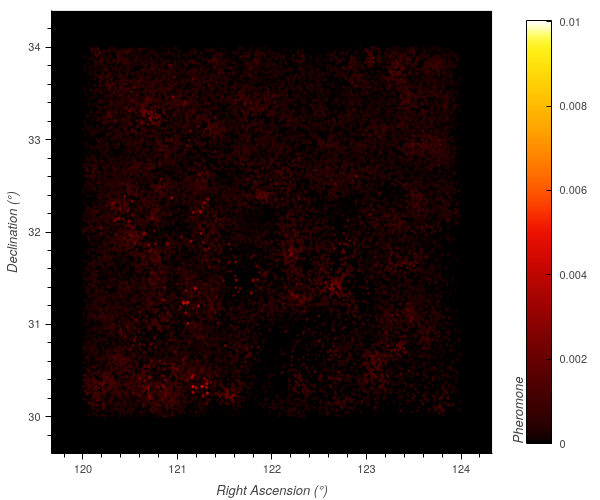
\includegraphics[width=\textwidth]{img/ant-colony-a1-120.0-30.0.png}
        \caption{\label{fig:ant-colony-dark-region}Dark Region}
    \end{subfigure}
    \hspace{-0.0225\textwidth}
    \begin{subfigure}[b]{0.335\textwidth}
        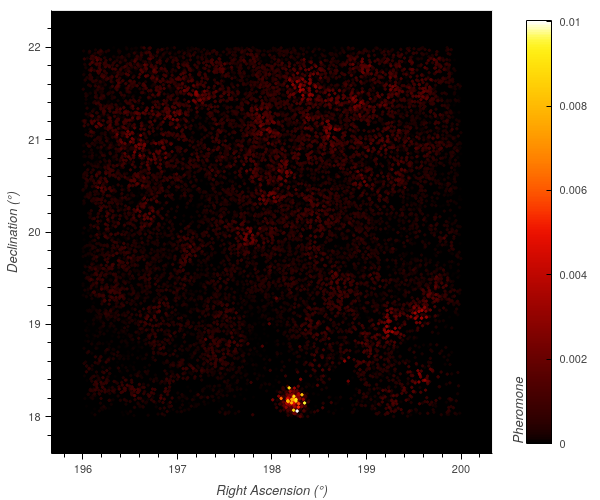
\includegraphics[width=\textwidth]{img/ant-colony-a1-196.0-18.0.png}
        \caption{\label{fig:ant-colony-one-blob}Dark Region with Bright Spot}
    \end{subfigure}
    \hspace{-0.0225\textwidth}
    \begin{subfigure}[b]{0.335\textwidth}
        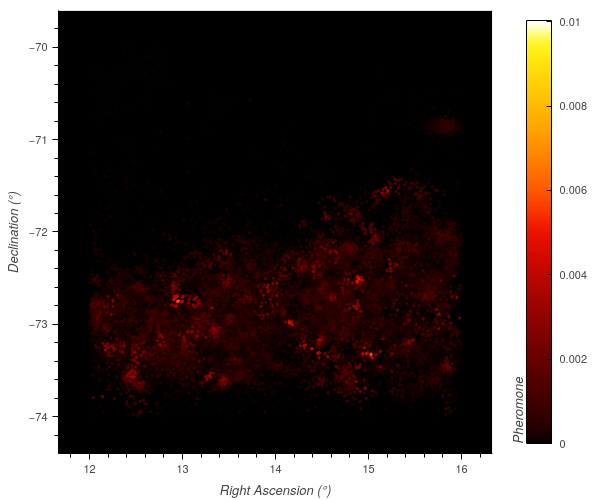
\includegraphics[width=\textwidth]{img/ant-colony-a3-12.0--74.0.png}
        \caption{\label{fig:ant-colony-bright-region}Bright Region}
    \end{subfigure}
    \caption{\label{fig:ant-colony-raster} Results of the Ant Colony Applied to the Three Types of Rasters}
\end{figure}
\vspace{-1.5em}
The brighter stars (yellow-white) correspond to stars with higher pheromone values than the darker stars (red-black). The rasters depicted in Figure~\ref{fig:ant-colony-dark-region} and Figure~\ref{fig:ant-colony-bright-region} are both relatively uniform with the first being mostly devoid of stars and the second being completely saturated with stars. As a result, it seems that the ants have not highlighted any major region of interest. However, for Figure~\ref{fig:ant-colony-one-blob} the ants have been able to pinpoint the cluster that is present within the raster. While, this cluster is apparent by eye alone, it is not always so evident from a pheromone heat-map that a cluster has been identified.

As a result, it is necessary to perform further processing to effectively extract potential clusters from the pheromone values. It is expected that the pheromone values within clusters will be high and the values outside of (and between clusters) will be low. This provides a boundary separating a cluster from other stellar structures. This forms the basis of the clustering algorithm.

\newpage{}
\section{\label{sec:Clustering}Gravitational Clustering Based on Pheromone Mapping}

The pheromone values encode the plethora of information related to the $\text{RA}$, $\text{Dec}$, $\text{Distance}$, $\text{PM}_{\text{RA}}$, and $\text{PM}_{\text{Dec}}$ of the stars. They provide a strong heuristic for identifying the boundaries between dense regions of similar stars. The next step is to then perform clustering such that stars with high pheromone values are grouped together. While the raw pheromone values do provide information on the density of the stars, it is quite possible for two stars in different but equally dense regions to have the same pheromone values. Thus, the clustering algorithm must also make use of the position of the star coupled with the pheromone values to determine which cluster a star may belong to.

To explain the clustering algorithm, it is necessary to reformulate the problem at hand. There are a number of points distributed in 3-dimensional space with a (pheromone) parameter attached to them that describes the strength of the attraction they feel to other points. In addition, points that are closer to each other should experience a stronger attractive force than points that are farther apart. This formulation reveals the similarity of this problem to the basic description of gravitational attraction. Newton's equation which governs gravitational attraction is as follows:
\begin{equation}
    F_{\text{gravity}} = g\frac{M_{x_{i}}M_{x_{j}}}{r^{2}}\label{eq:gravitational-attraction}
\end{equation}
\indent{}In Eq.~\eqref{eq:gravitational-attraction}, $g$ represents the gravitational constant, $M_{x}$ represents the mass of some object $x$, and $r$ represents the distance between the \textit{center-of-gravity} (CoG) of $x_{i}$ and $x_{j}$. The clustering algorithm uses this as its foundation but uses the pheromone values in place of the mass to determine the attraction between the stars. Stars which are sufficiently attracted to each other will pool to form a cluster which in turn may continue to grow and attract more stars.

\subsection{Components of the Clustering Algorithm}
In the pheromone-based gravitational clustering, an initial cluster will form out of single star. Stars within the field of attraction of this cluster will be absorbed. The  strength of this attraction is based on the pheromone mass of both the cluster and the star and is defined as follows:
\begin{align}
    P_{x_{i}}                       & = \mathbf{f}[x_{i}]                          & \parbox[t]{0.4\textwidth}{\textit{The pheromone mass for a single star.}} \\
    P_{C}                           & = \sum\limits_{x_{k} \in C}\mathbf{f}[x_{k}] & \parbox[t]{0.4\textwidth}{\textit{The pheromone mass for a cluster.}}     \\
    \hphantom{F_{\text{pheromone}}} & \hphantom{= \frac{P_{C}P_{x_{i}}}{r^{2}}}    & \nonumber{}
\end{align}
\\
\vspace{-4.5em}

\noindent The force of attraction between the cluster ($C$) and the star ($x_{i}$) is then defined as follows:
\begin{align}
    F_{\text{pheromone}} & = \frac{P_{C}P_{x_{i}}}{r^{2}}                          & \parbox[t]{0.4\textwidth}{\textit{The pheromone attraction force between a cluster $C$ and a star $x_{i}$.}} \label{eq:pheromone-force} \\
    \hphantom{P_{C}}     & \hphantom{= \sum\limits_{x_{k} \in C}\mathbf{f}[x_{k}]} & \nonumber{}
\end{align}
\\
\vspace{-5.0em}

\noindent{}%
In Eq.~\eqref{eq:pheromone-force}:
\begin{itemize}
    \item $P_{C}$ represents the pheromone mass of the cluster $C$.
    \item $P_{x_{i}}$ represents the pheromone mass of some star $x_{i}$.
    \item $r$ represents the Euclidean distance between the CoG of the cluster $C$ and the star $x_{i}$.
\end{itemize}
This is effective for stars with a $\text{pheromone value} > 0$. However, across a given raster there may be stars that were never visited by the ants. These stars would have a $\text{pheromone value} = 0$ and even if they were geometrically contained within a cluster, by Eq.~\eqref{eq:pheromone-force} they would have an attraction force equal to zero. So, stars with a non-zero pheromone value should be clustered differently than stars with a zero pheromone value. Thus, the basic algorithm for the pheromone clustering, Alg.\,\ref{alg:pheromone-clustering}, is composed of these two steps as well as a final filtration step based on a minimum accepted number of stars contained within a GC, ${N_{\text{GC}}}_{\text{min}}$ (see Section~\ref{sec:constants} for the value that was selected).
\vspace{-0.5em}
\begin{algorithm}[H]
    \caption{\label{alg:pheromone-clustering}Pheromone Clustering}
    \footnotesize{}
    \begin{algorithmic}
        \Require{
            \vspace{-1.55em}
            \begin{itemize}
                \item The stars where for each star, $x_{i}$ the following are available: $\text{RA}_{x_{i}}$, $\text{Dec}_{x_{i}}$, and $\text{Distance}_{x_{i}}$.
                \item The pheromone values for the stars, $\mathbf{f}$ where for some star, $x_{i}$ its pheromone value may be accessed by $\mathbf{f}[x_{i}]$.
            \end{itemize}
        }
        \Ensure{The set of clusters present across the stars.}

        \begin{minipage}{\columnwidth{}}
            \hspace{-5em}
            \vhrulefill{0.3pt}
        \end{minipage}
        \State{$(\text{stars}_{\mathbf{f} = 0}, \text{stars}_{\mathbf{f}\neq0}) \gets \text{Partition stars by $\mathbf{f}$}$}
        \Comment{Stars with a zero pheromone value must be processed separately.}
        \State{$\text{clusters}_{\text{initial}} \gets \text{Cluster the stars with non-zero pheromone values using Alg.\,\ref{alg:non-zero-clustering}}$}
        \Comment{This uses $\text{stars}_{f \neq 0}$.}
        \State{$\text{clusters}_{\text{all}} \gets \text{Cluster the stars with zero pheromone values using Alg.\,\ref{alg:zero-clustering}}$}
        \Comment{This uses $\text{clusters}_{\text{initial}}$ and $\text{stars}_{f = 0}$.}
        \State{$\text{clusters}_{\text{filtered}} \gets \text{Filter out clusters from $\text{clusters}_{\text{all}}$ that contain fewer than ${N_{\text{GC}}}_{\text{min}}$ stars}$}
        \State{\Return{$\text{clusters}_{\text{filtered}}$}}
    \end{algorithmic}
\end{algorithm}

To perform the clustering using the non-zero pheromone values it is necessary to compute the center-of-gravity based on these pheromone values. The equation for this is as follows:
\vspace{-0.35em}
\begin{align}
    \text{CoG}_{C} = \tfrac{\mathlarger{\sum\limits_{x_{i} \in C}}\Bigl(\text{position}_{x_{i}} \times P_{x_{i}}\Bigr)}{\abs{C} \times \mathlarger{\sum\limits_{x_{i} \in C}}P_{x_{i}}} \label{eq:cog}
\end{align}
The $\text{CoG}_{C}$ is the average position of the stars in $C$ where the contribution of each star is weighted by their pheromone mass. This provides a coordinate in $(\text{RA}, \text{Dec}, \text{Distance})$ which may then be used as part of the non-zero pheromone clustering.
\vspace{-0.5em}
\begin{algorithm}[H]
    \caption{\label{alg:non-zero-clustering}Non-Zero Pheromone Clustering}
    \footnotesize{}
    \begin{algorithmic}
        \Require{The stars with non-zero pheromone values ($\text{stars}_{\mathbf{f} \neq 0}$)}
        \Ensure{The clusters from $\text{stars}_{\mathbf{f} \neq 0}$}

        \begin{minipage}{\columnwidth{}}
            \hspace{-5em}
            \vhrulefill{0.3pt}
        \end{minipage}
        \State{$\text{clusters} \gets \text{Create an empty set to contain the clusters that are found}$}
        \State{$\text{stars}_{\text{to process}} = \text{stars}_{\mathbf{f} \neq 0}$}
        \While{$\text{stars}_{\text{to process}}$ is not empty}
        \State{$C \gets \text{Create an empty cluster}$}
        \State{$\text{star} \gets \text{Pop the star with the greatest pheromone value from $\text{stars}_{\text{to process}}$}$}
        \State{Insert $\text{star}$ in $C$}
        \Repeat{}
        \State{$\text{cluster}_{\text{changed}} = \tx{false}$}
        \ForAll{$x_{i} \in \text{star}_{\text{to process}}$}
        \State{$\text{CoG}_{C} \gets \text{Compute the center-of-gravity of $C$ using Eq.~\eqref{eq:cog}}$}
        \State{$r \gets \text{Compute the Euclidean distance between $\text{CoG}_{C}$ and the position of $x_{i}$}$}
        \State{$F_{\text{pheromone}} = \dfrac{P_{C}P_{x_{i}}}{r^{2}}$}
        \Comment{Based on Eq.~\eqref{eq:pheromone-force}.}
        \If{$F_{\text{pheromone}} \geq F_{\text{min attraction}}$}
        \State{Remove $x_{i}$ from $\text{stars}_{\text{to process}}$}
        \State{Insert $x_{i}$ in $C$}
        \State{$\text{cluster}_{\text{changed}} = \tx{true}$}
        \EndIf{}
        \EndFor{}
        \Until{$\text{cluster}_{\text{changed}} == \tx{false}$}
        \State{Insert $C$ in $\text{clusters}$}
        \EndWhile{}
        \State{\Return{clusters}}
    \end{algorithmic}
\end{algorithm}
\vspace{-1.35em}
\indent{}In this algorithm, every star under consideration is added to a list of stars to be processed. While stars remain to be processed, a cluster is generated and populated with the star with the highest pheromone mass of the stars that remain. Then this cluster is grown within the \tx{repeat-until} loop until the cluster ceases to grow. Within this loop all the stars that remain have their position compared with the center-of-gravity of the cluster.

The resulting distance is then used alongside the pheromone mass of the star and the cluster to compute the pheromone attractive force ($F_{\text{pheromone}}$). If this force is sufficiently high the star is absorbed into the cluster, thereby increasing the pheromone mass of the cluster and shifting its center-of-gravity. These clusters are generated and grown repeatedly in this fashion until every star has been assigned to a cluster (even if it is simply a cluster containing that one star).

After this algorithm has run all potential clusters are now found. It is now necessary to incorporate the stars with the zero pheromone values whose positions overlap with the clusters. In essence these stars correspond to objects without a \textit{gravitational} field. Thus, it is necessary to consult the centroid of the clusters instead of their center-of-gravity.
\vspace{-0.21em}
\begin{align}
    \text{centroid}_{C} = \tfrac{\mathlarger{\sum\limits_{x_{i} \in C}}\text{position}_{x_{i}}}{\abs{C}} \label{eq:centroid}
\end{align}
The centroid is the average position of the stars in $C$. With this, the zero pheromone clustering is:
\vspace{-1.75em}
\begin{algorithm}[H]
    \caption{\label{alg:zero-clustering}Zero Pheromone Clustering}
    \footnotesize{}
    \begin{algorithmic}
        \Require{
            \vspace{-1.55em}
            \begin{itemize}
                \item The stars with zero pheromone values ($\text{stars}_{\mathbf{f}=0}$)
                \item The clusters based on the initial non-zero clustering from Alg.\,\ref{alg:non-zero-clustering} ($\text{clusters}_{\text{initial}}$)
            \end{itemize}
        }
        \Ensure{The clusters incorporating $\text{stars}_{\mathbf{f} = 0}$ across $\text{clusters}_{\text{initial}}$}

        \begin{minipage}{\columnwidth{}}
            \hspace{-5em}
            \vhrulefill{0.3pt}
        \end{minipage}
        \State{$\text{clusters}_{\text{all}} = \text{clusters}_{\text{initial}}$}
        \ForAll{$x_i \in \text{stars}_{\mathbf{f} = 0}$}
        \State{$\text{clusters}_{\text{closest}} \gets \text{clusters}_{\text{all}} \text{ sorted in ascending order by Euclidean distance from centroid of cluster to } x_{i}$}
        \BeginBox[draw=blue, dashed]{}
        \ForAll{$\text{cluster} \in \text{clusters}_{\text{closest}}$}
        \EndBox{}
        % \If{$x_{i}$ is within the bounds of the stars of the cluster}
        \If{
            \fcolorbox{black}{lightgray}{%
                \begin{minipage}{0.43\columnwidth{}}
                    $
                        \begin{aligned}
                             & {C_{\text{RA}}}_{\text{min}} \leq \text{RA}_{x_i} \leq {C_{\text{RA}}}_{\text{max}} \land{}                       \\
                             & \hspace{1em}{C_{\text{Dec}}}_{\text{min}} \leq \text{Dec}_{x_i} \leq {C_{\text{Dec}}}_{\text{max}} \land{}        \\
                             & \hspace{2em}{C_{\text{Distance}}}_{\text{min}} \leq \text{Distance}_{x_i} \leq {C_{\text{Distance}}}_{\text{max}}
                        \end{aligned}
                    $
                \end{minipage}%
            }
        }
        \Comment{Check if $x_{i}$ is within the bounds of the cluster.}
        % \If{$x_{i}$ is within the bounds of the stars of the cluster}
        \State{Insert $x_{i}$ into the cluster}
        \Break{\hspace{0.65em}\BoxedString[draw=blue, dashed]{Out of inner loop}}
        \EndIf{}
        \EndFor{}
        \EndFor{}
        \State{\Return{$\text{clusters}_{\text{all}}$}}
    \end{algorithmic}
\end{algorithm}

In the zero pheromone clustering, each star in the set of zero pheromone stars is considered. The preexisting clusters are then searched through in order of closest to farthest based on the Euclidean distance between the centroid of the cluster and the position of the star. The star is then absorbed by the first cluster that has the star within its bounds. If no cluster contains the star it is simply left unclustered.

\subsection{Interpreting the Results of the Clustering}
With all these steps in tow, the results are a set of clusters each of which contain a set of stars. The information of these stars within the clusters may be plotted alongside the rest of the stars to provide a visualization of the clusters contained within a raster. Of the three exemplar rasters, only the dark region with the bright spot shown in Figure~\ref{fig:dark-region-bright-spot} is identified as containing clusters. A 2-dimensional plot of the pheromone heat-map and the clustering of the raster may be seen in Figure~\ref{fig:example-2d-cluster}.
\begin{figure}[H]
    \centering
    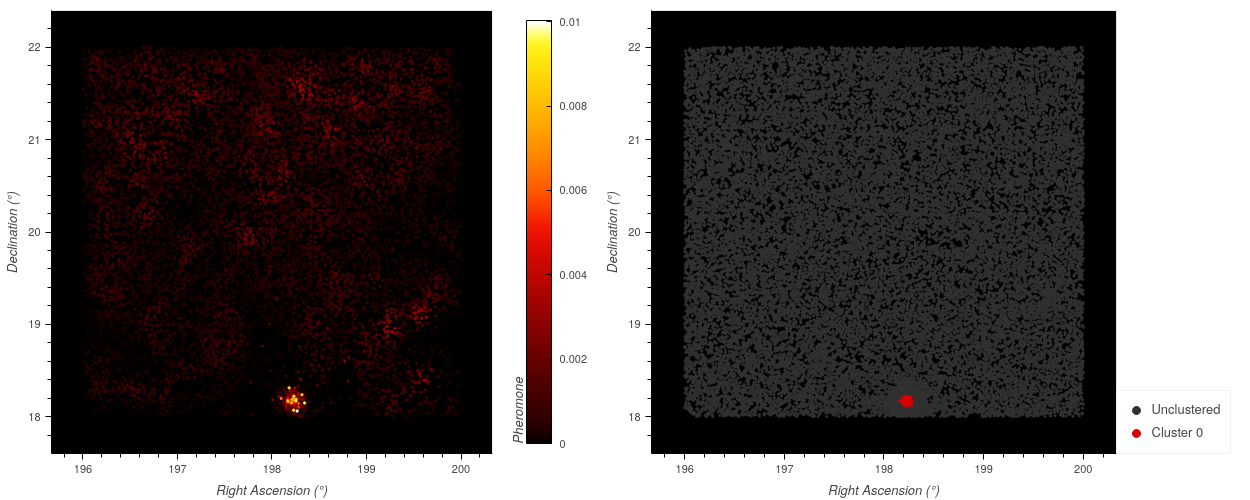
\includegraphics[width=1.1\textwidth]{img/2d-clustering-a1-196.0-18.0.png}
    \caption{\label{fig:example-2d-cluster} Clustering of Dark Region with Bright Spot}
\end{figure}
Additionally, in this instance only one cluster is identified. However, it is possible for multiple clusters to be involved and for these clusters to overlap in $\text{RA}$ and $\text{Dec}$. To provide visualization in such cases 3-dimensional plots have also been used, such as the plot in Figure~\ref{fig:example-3d-cluster} which focuses the region containing the GC.
\vspace{-1em}
\begin{figure}[H]
    \centering
    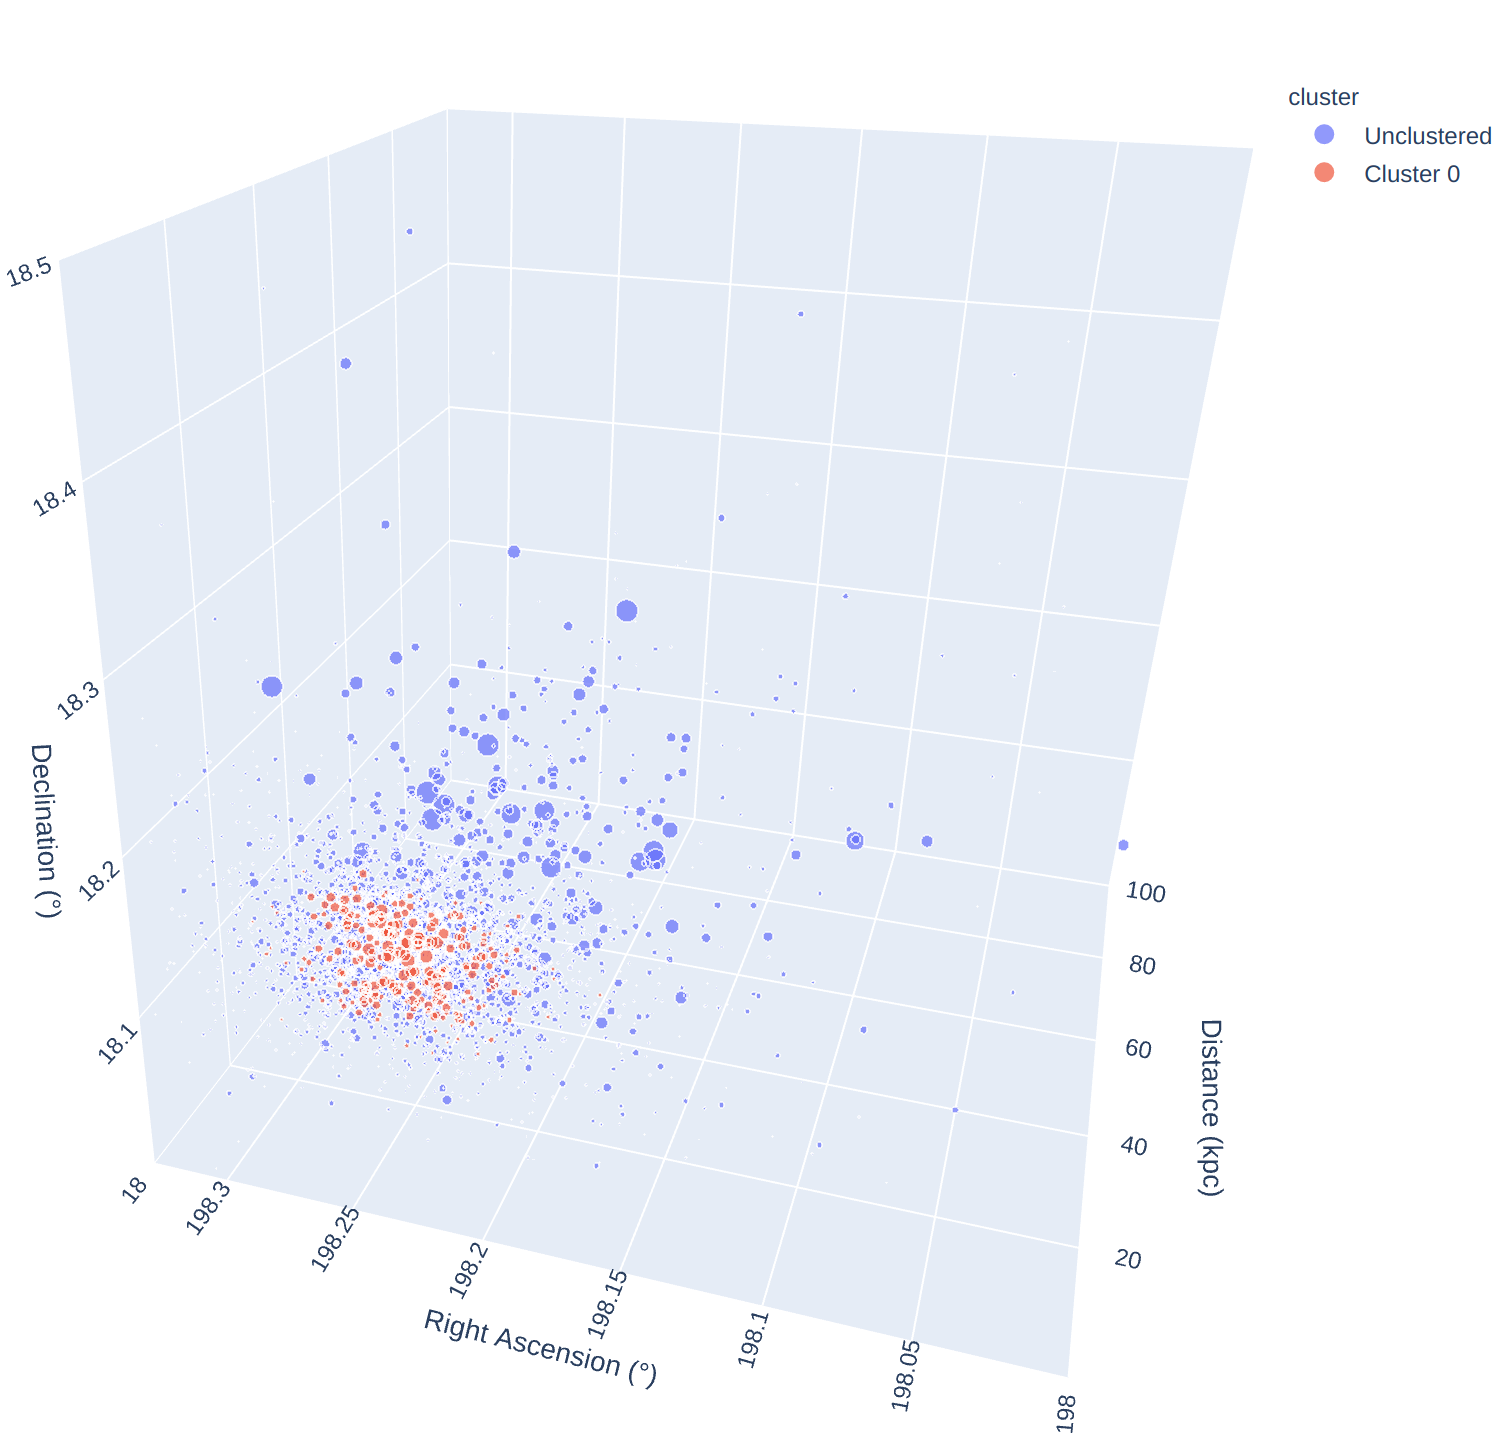
\includegraphics[width=0.65\textwidth]{img/clusters.png}
    \caption{\label{fig:example-3d-cluster} 3D Plot of Cluster in Dark Region with Bright Spot}
\end{figure}

\newpage{}

\section{\label{sec:constants}Constants}
There are a variety of constants whose values impact the functioning of the pipeline. They are presented in Table~\ref{tb:constants} with their descriptions, their values, and how those values were determined.
\begin{table}[H]
    \centering
    \caption{All Constants}
    \label{tb:constants}
    \resizebox{\textwidth}{!}{%
        \renewcommand{\arraystretch}{1.8}
        \begin{tabular}{l l l p{10cm}}
            \toprule
            Name                           & Value & Algorithm  & Explanation                                                                                                                                                                                                                                                                                                                                                                                                                                                                                                                                                                                        \\
            \midrule
            $B_{\text{threshold}}$         & 0.2   & \blobdog{} & This threshold represents the smallest blob scale that should be considered a valid blob. The value for this constant was determined through experimentation described in Table~\ref{tb:number-of-remaining-rasters}.                                                                                                                                                                                                                                                                                                                                                                              \\

            $N_{\text{gens}}$              & 5     & Ant Colony & Number of generations in the execution of the Ant Colony algorithm. Each generation incorporates the results of the previous generation to uncover network substructure. This  value was set based on work by Mohammadi on the Ant Colony algorithm~\cite{AntColonyMohammadi}. Future experimentation should be done to optimize this value.                                                                                                                                                                                                                                                       \\

            $N_{\text{ants}}$              & 30    & Ant Colony & Number of ants exploring a given raster across a single generation. This  value was set based on work by Mohammadi on the Ant Colony algorithm~\cite{AntColonyMohammadi}. Future experimentation should be done to optimize this value.                                                                                                                                                                                                                                                                                                                                                            \\

            $N_{\text{steps}}$             & 2000  & Ant Colony & Number of steps each ant is allowed to take across a given generation. This value was set based on work by Mohammadi on the Ant Colony algorithm~\cite{AntColonyMohammadi}. Future experimentation should be done to optimize this value.                                                                                                                                                                                                                                                                                                                                                          \\

            $N_{\text{neighbors}}$         & 20    & Ant Colony & The number of neighbors an ant should consider when transitioning between stars during one step. This is an optimization taking advantage of the fact that the ants' choice of their next star is weighted in part by the distance to that star from the current star. Setting this parameter too low will prevent the ants from spontaneously considering stars further afield. Setting it too high will simply increase the time taken for the execution of the algorithm. This value was determined through trial-and-error and should be experimented on further to identify the lowest bound. \\

            $\gamma$                       & 0.9   & Ant Colony & This value represents a ratio in the mixture of the pre-existing pheromone values from previous generations and the results from the current generation. At $\gamma = 1$, the ants only incorporate the results of the current generation in determining their next transition. At $\gamma = 0$, the ants only incorporate the results from the previous generation in determining their next transition. This value was set based on work by Mohammadi on the Ant Colony algorithm~\cite{AntColonyMohammadi}. Future experimentation should be done to optimize this value.                       \\

            $\rho$                         & 0.1   & Ant Colony & Across each generation of the Ant Colony algorithm the pheromone values from the previous generation are combined with the results of the current generation. This parameter controls how strong of an influence the previous pheromone values are on the new pheromone values. A value of $0$ means that the previous pheromone values do not contribute to the new pheromone values. This value was set based on the work by Mohammadi on the Ant Colony~\cite{AntColonyMohammadi} and requires further experimentation.                                                                         \\

            $F_{\text{min attraction}}$    & 0.01  & Clustering & The minimum force constituting a valid attraction between concentrations of pheromone mass. This value was determined through trial-and-error and should face more thorough experimentation in the future.                                                                                                                                                                                                                                                                                                                                                                                         \\
            ${N_{\text{GC}}}_{\text{min}}$ & 100   & Clustering & Each cluster identified by the clustering contains a set of stars. This value represents the minimum number of stars that should be present in the set for it to be considered a valid cluster and maintained. The smallest stellar cluster consists of 100 stars~\cite{Dugan2019} and thus this was used as the value.                                                                                                                                                                                                                                                                            \\
            \bottomrule
        \end{tabular}
    }
\end{table}
\renewcommand{\arraystretch}{1}
